%%%%%%%%%%%%%%%%%%%%%%%%%%%%%%%%%%%%%%%%%
% Masters/Doctoral Thesis
% LaTeX Template
% Version 2.5 (27/8/17)
%
% This template was downloaded from:
% http://www.LaTeXTemplates.com
%
% Version 2.x major modifications by:
% Vel (vel@latextemplates.com)
%
% This template is based on a template by:
% Steve Gunn (http://users.ecs.soton.ac.uk/srg/softwaretools/document/templates/)
% Sunil Patel (http://www.sunilpatel.co.uk/thesis-template/)
%
% Template license:
% CC BY-NC-SA 3.0 (http://creativecommons.org/licenses/by-nc-sa/3.0/)
%
%%%%%%%%%%%%%%%%%%%%%%%%%%%%%%%%%%%%%%%%%

%----------------------------------------------------------------------------------------
%	PACKAGES AND OTHER DOCUMENT CONFIGURATIONS
%----------------------------------------------------------------------------------------

\documentclass[
11pt, % The default document font size, options: 10pt, 11pt, 12pt
%oneside, % Two side (alternating margins) for binding by default, uncomment to switch to one side
ngerman, % ngerman for German
singlespacing, % Single line spacing, alternatives: onehalfspacing or doublespacing
%draft, % Uncomment to enable draft mode (no pictures, no links, overfull hboxes indicated)
%nolistspacing, % If the document is onehalfspacing or doublespacing, uncomment this to set spacing in lists to single
liststotoc, % Uncomment to add the list of figures/tables/etc to the table of contents
%toctotoc, % Uncomment to add the main table of contents to the table of contents
%parskip, % Uncomment to add space between paragraphs
%nohyperref, % Uncomment to not load the hyperref package
headsepline, % Uncomment to get a line under the header
%chapterinoneline, % Uncomment to place the chapter title next to the number on one line
%consistentlayout, % Uncomment to change the layout of the declaration, abstract and acknowledgements pages to match the default layout
]{MastersDoctoralThesis} % The class file specifying the document structure

\usepackage[utf8]{inputenc} % Required for inputting international characters
\usepackage[T1]{fontenc} % Output font encoding for international characters

\usepackage{mathpazo} % Use the Palatino font by default

\usepackage[backend=bibtex,style=authoryear,natbib=true]{biblatex} % Use the bibtex backend with the authoryear citation style (which resembles APA)

%\addbibresource{example.bib} % The filename of the bibliography

\usepackage[autostyle=true]{csquotes} % Required to generate language-dependent quotes in the bibliography

%----------------------------------------------------------------------------------------
%	MARGIN SETTINGS
%----------------------------------------------------------------------------------------

\geometry{
	paper=a4paper, % Change to letterpaper for US letter
	inner=2.5cm, % Inner margin
	outer=3.8cm, % Outer margin
	bindingoffset=.5cm, % Binding offset
	top=1.5cm, % Top margin
	bottom=1.5cm, % Bottom margin
	%showframe, % Uncomment to show how the type block is set on the page
}

\providecommand{\tightlist}{%
  \setlength{\itemsep}{0pt}\setlength{\parskip}{0pt}}

%----------------------------------------------------------------------------------------
%	THESIS INFORMATION
%----------------------------------------------------------------------------------------

\thesistitle{Konzertkalender} % Your thesis title, this is used in the title and abstract, print it elsewhere with \ttitle
\supervisor{Sandro Bertolino} % Your supervisor's name, this is used in the title page, print it elsewhere with \supname
\examiner{} % Your examiner's name, this is not currently used anywhere in the template, print it elsewhere with \examname
\degree{Dipl. Techniker Informatik} % Your degree name, this is used in the title page and abstract, print it elsewhere with \degreename
\author{Damian \textsc{Senn}} % Your name, this is used in the title page and abstract, print it elsewhere with \authorname
\addresses{} % Your address, this is not currently used anywhere in the template, print it elsewhere with \addressname

\subject{} % Your subject area, this is not currently used anywhere in the template, print it elsewhere with \subjectname
\keywords{} % Keywords for your thesis, this is not currently used anywhere in the template, print it elsewhere with \keywordnames
\university{\href{http://www.tsbe.ch}{TSBE}} % Your university's name and URL, this is used in the title page and abstract, print it elsewhere with \univname
\department{} % Your department's name and URL, this is used in the title page and abstract, print it elsewhere with \deptname
\group{} % Your research group's name and URL, this is used in the title page, print it elsewhere with \groupname
\faculty{} % Your faculty's name and URL, this is used in the title page and abstract, print it elsewhere with \facname

\AtBeginDocument{
\hypersetup{pdftitle=\ttitle} % Set the PDF's title to your title
\hypersetup{pdfauthor=\authorname} % Set the PDF's author to your name
\hypersetup{pdfkeywords=\keywordnames} % Set the PDF's keywords to your keywords
}

\begin{document}

\frontmatter % Use roman page numbering style (i, ii, iii, iv...) for the pre-content pages

\pagestyle{plain} % Default to the plain heading style until the thesis style is called for the body content

%----------------------------------------------------------------------------------------
%	TITLE PAGE
%----------------------------------------------------------------------------------------

\begin{titlepage}
\begin{center}

\vspace*{.06\textheight}
{\scshape\LARGE \univname\par}\vspace{1.5cm} % University name
\textsc{\Large Diplomarbeit}\\[0.5cm] % Thesis type

\HRule \\[0.4cm] % Horizontal line
{\huge \bfseries \ttitle\par}\vspace{0.4cm} % Thesis title
\HRule \\[1.5cm] % Horizontal line

\begin{minipage}[t]{0.4\textwidth}
\begin{flushleft} \large
\emph{Author:}\\
\href{mailto:damian.senn@gmail.com}{\authorname} % Author name - remove the \href bracket to remove the link
\end{flushleft}
\end{minipage}
\begin{minipage}[t]{0.4\textwidth}
\begin{flushright} \large
\emph{Experten:} \\
\href{mailto:sandro@bertolino.ch}{\supname}\\
\href{mailto:raez@puzzle.ch}{Severin Räz}
\end{flushright}
\end{minipage}\\[3cm]

\vfill

\large \textit{Eine Diplomarbeit für den Abschluss \degreename}\\[0.3cm] % University requirement text

\vfill

{\large \today}\\[4cm] % Date
%\includegraphics{Logo} % University/department logo - uncomment to place it

\vfill
\end{center}
\end{titlepage}

%----------------------------------------------------------------------------------------
%	DECLARATION PAGE
%----------------------------------------------------------------------------------------

\begin{declaration}
\addchaptertocentry{\authorshipname} % Add the declaration to the table of contents
\noindent I, \authorname, declare that this thesis titled, \enquote{\ttitle} and the work presented in it are my own. I confirm that:

\begin{itemize}
\item This work was done wholly or mainly while in candidature for a research degree at this University.
\item Where any part of this thesis has previously been submitted for a degree or any other qualification at this University or any other institution, this has been clearly stated.
\item Where I have consulted the published work of others, this is always clearly attributed.
\item Where I have quoted from the work of others, the source is always given. With the exception of such quotations, this thesis is entirely my own work.
\item I have acknowledged all main sources of help.
\item Where the thesis is based on work done by myself jointly with others, I have made clear exactly what was done by others and what I have contributed myself.\\
\end{itemize}

\noindent Signed:\\
\rule[0.5em]{25em}{0.5pt} % This prints a line for the signature

\noindent Date:\\
\rule[0.5em]{25em}{0.5pt} % This prints a line to write the date
\end{declaration}

\cleardoublepage

%----------------------------------------------------------------------------------------
%	ABSTRACT PAGE
%----------------------------------------------------------------------------------------

\begin{abstract}
\addchaptertocentry{\abstractname} % Add the abstract to the table of contents
The Thesis Abstract is written here (and usually kept to just this page). The page is kept centered vertically so can expand into the blank space above the title too\ldots
\end{abstract}

%----------------------------------------------------------------------------------------
%	ACKNOWLEDGEMENTS
%----------------------------------------------------------------------------------------

\begin{acknowledgements}
\addchaptertocentry{\acknowledgementname} % Add the acknowledgements to the table of contents
The acknowledgments and the people to thank go here, don't forget to include your project advisor\ldots
\end{acknowledgements}

%----------------------------------------------------------------------------------------
%	LIST OF CONTENTS/FIGURES/TABLES PAGES
%----------------------------------------------------------------------------------------

\tableofcontents % Prints the main table of contents

\listoffigures % Prints the list of figures

\listoftables % Prints the list of tables

%----------------------------------------------------------------------------------------
%	ABBREVIATIONS
%----------------------------------------------------------------------------------------

\begin{abbreviations}{ll} % Include a list of abbreviations (a table of two columns)

\textbf{LAH} & \textbf{L}ist \textbf{A}bbreviations \textbf{H}ere\\
\textbf{WSF} & \textbf{W}hat (it) \textbf{S}tands \textbf{F}or\\

\end{abbreviations}

%----------------------------------------------------------------------------------------
%	DEDICATION
%----------------------------------------------------------------------------------------

\dedicatory{For/Dedicated to/To my\ldots}

%----------------------------------------------------------------------------------------
%	THESIS CONTENT - CHAPTERS
%----------------------------------------------------------------------------------------

\mainmatter % Begin numeric (1,2,3...) page numbering

\pagestyle{thesis} % Return the page headers back to the "thesis" style

% Include the chapters of the thesis as separate files from the Chapters folder
% Uncomment the lines as you write the chapters

%% Chapter 1

\chapter{Chapter Title Here} % Main chapter title

\label{Chapter1} % For referencing the chapter elsewhere, use \ref{Chapter1} 

%----------------------------------------------------------------------------------------

% Define some commands to keep the formatting separated from the content 
\newcommand{\keyword}[1]{\textbf{#1}}
\newcommand{\tabhead}[1]{\textbf{#1}}
\newcommand{\code}[1]{\texttt{#1}}
\newcommand{\file}[1]{\texttt{\bfseries#1}}
\newcommand{\option}[1]{\texttt{\itshape#1}}

%----------------------------------------------------------------------------------------

\section{Welcome and Thank You}
Welcome to this \LaTeX{} Thesis Template, a beautiful and easy to use template for writing a thesis using the \LaTeX{} typesetting system.

If you are writing a thesis (or will be in the future) and its subject is technical or mathematical (though it doesn't have to be), then creating it in \LaTeX{} is highly recommended as a way to make sure you can just get down to the essential writing without having to worry over formatting or wasting time arguing with your word processor.

\LaTeX{} is easily able to professionally typeset documents that run to hundreds or thousands of pages long. With simple mark-up commands, it automatically sets out the table of contents, margins, page headers and footers and keeps the formatting consistent and beautiful. One of its main strengths is the way it can easily typeset mathematics, even \emph{heavy} mathematics. Even if those equations are the most horribly twisted and most difficult mathematical problems that can only be solved on a super-computer, you can at least count on \LaTeX{} to make them look stunning.

%----------------------------------------------------------------------------------------

\section{Learning \LaTeX{}}

\LaTeX{} is not a \textsc{wysiwyg} (What You See is What You Get) program, unlike word processors such as Microsoft Word or Apple's Pages. Instead, a document written for \LaTeX{} is actually a simple, plain text file that contains \emph{no formatting}. You tell \LaTeX{} how you want the formatting in the finished document by writing in simple commands amongst the text, for example, if I want to use \emph{italic text for emphasis}, I write the \verb|\emph{text}| command and put the text I want in italics in between the curly braces. This means that \LaTeX{} is a \enquote{mark-up} language, very much like HTML.

\subsection{A (not so short) Introduction to \LaTeX{}}

If you are new to \LaTeX{}, there is a very good eBook -- freely available online as a PDF file -- called, \enquote{The Not So Short Introduction to \LaTeX{}}. The book's title is typically shortened to just \emph{lshort}. You can download the latest version (as it is occasionally updated) from here:
\url{http://www.ctan.org/tex-archive/info/lshort/english/lshort.pdf}

It is also available in several other languages. Find yours from the list on this page: \url{http://www.ctan.org/tex-archive/info/lshort/}

It is recommended to take a little time out to learn how to use \LaTeX{} by creating several, small `test' documents, or having a close look at several templates on:\\ 
\url{http://www.LaTeXTemplates.com}\\ 
Making the effort now means you're not stuck learning the system when what you \emph{really} need to be doing is writing your thesis.

\subsection{A Short Math Guide for \LaTeX{}}

If you are writing a technical or mathematical thesis, then you may want to read the document by the AMS (American Mathematical Society) called, \enquote{A Short Math Guide for \LaTeX{}}. It can be found online here:
\url{http://www.ams.org/tex/amslatex.html}
under the \enquote{Additional Documentation} section towards the bottom of the page.

\subsection{Common \LaTeX{} Math Symbols}
There are a multitude of mathematical symbols available for \LaTeX{} and it would take a great effort to learn the commands for them all. The most common ones you are likely to use are shown on this page:
\url{http://www.sunilpatel.co.uk/latex-type/latex-math-symbols/}

You can use this page as a reference or crib sheet, the symbols are rendered as large, high quality images so you can quickly find the \LaTeX{} command for the symbol you need.

\subsection{\LaTeX{} on a Mac}
 
The \LaTeX{} distribution is available for many systems including Windows, Linux and Mac OS X. The package for OS X is called MacTeX and it contains all the applications you need -- bundled together and pre-customized -- for a fully working \LaTeX{} environment and work flow.
 
MacTeX includes a custom dedicated \LaTeX{} editor called TeXShop for writing your `\file{.tex}' files and BibDesk: a program to manage your references and create your bibliography section just as easily as managing songs and creating playlists in iTunes.

%----------------------------------------------------------------------------------------

\section{Getting Started with this Template}

If you are familiar with \LaTeX{}, then you should explore the directory structure of the template and then proceed to place your own information into the \emph{THESIS INFORMATION} block of the \file{main.tex} file. You can then modify the rest of this file to your unique specifications based on your degree/university. Section \ref{FillingFile} on page \pageref{FillingFile} will help you do this. Make sure you also read section \ref{ThesisConventions} about thesis conventions to get the most out of this template.

If you are new to \LaTeX{} it is recommended that you carry on reading through the rest of the information in this document.

Before you begin using this template you should ensure that its style complies with the thesis style guidelines imposed by your institution. In most cases this template style and layout will be suitable. If it is not, it may only require a small change to bring the template in line with your institution's recommendations. These modifications will need to be done on the \file{MastersDoctoralThesis.cls} file.

\subsection{About this Template}

This \LaTeX{} Thesis Template is originally based and created around a \LaTeX{} style file created by Steve R.\ Gunn from the University of Southampton (UK), department of Electronics and Computer Science. You can find his original thesis style file at his site, here:
\url{http://www.ecs.soton.ac.uk/~srg/softwaretools/document/templates/}

Steve's \file{ecsthesis.cls} was then taken by Sunil Patel who modified it by creating a skeleton framework and folder structure to place the thesis files in. The resulting template can be found on Sunil's site here:
\url{http://www.sunilpatel.co.uk/thesis-template}

Sunil's template was made available through \url{http://www.LaTeXTemplates.com} where it was modified many times based on user requests and questions. Version 2.0 and onwards of this template represents a major modification to Sunil's template and is, in fact, hardly recognisable. The work to make version 2.0 possible was carried out by \href{mailto:vel@latextemplates.com}{Vel} and Johannes Böttcher.

%----------------------------------------------------------------------------------------

\section{What this Template Includes}

\subsection{Folders}

This template comes as a single zip file that expands out to several files and folders. The folder names are mostly self-explanatory:

\keyword{Appendices} -- this is the folder where you put the appendices. Each appendix should go into its own separate \file{.tex} file. An example and template are included in the directory.

\keyword{Chapters} -- this is the folder where you put the thesis chapters. A thesis usually has about six chapters, though there is no hard rule on this. Each chapter should go in its own separate \file{.tex} file and they can be split as:
\begin{itemize}
\item Chapter 1: Introduction to the thesis topic
\item Chapter 2: Background information and theory
\item Chapter 3: (Laboratory) experimental setup
\item Chapter 4: Details of experiment 1
\item Chapter 5: Details of experiment 2
\item Chapter 6: Discussion of the experimental results
\item Chapter 7: Conclusion and future directions
\end{itemize}
This chapter layout is specialised for the experimental sciences, your discipline may be different.

\keyword{Figures} -- this folder contains all figures for the thesis. These are the final images that will go into the thesis document.

\subsection{Files}

Included are also several files, most of them are plain text and you can see their contents in a text editor. After initial compilation, you will see that more auxiliary files are created by \LaTeX{} or BibTeX and which you don't need to delete or worry about:

\keyword{example.bib} -- this is an important file that contains all the bibliographic information and references that you will be citing in the thesis for use with BibTeX. You can write it manually, but there are reference manager programs available that will create and manage it for you. Bibliographies in \LaTeX{} are a large subject and you may need to read about BibTeX before starting with this. Many modern reference managers will allow you to export your references in BibTeX format which greatly eases the amount of work you have to do.

\keyword{MastersDoctoralThesis.cls} -- this is an important file. It is the class file that tells \LaTeX{} how to format the thesis. 

\keyword{main.pdf} -- this is your beautifully typeset thesis (in the PDF file format) created by \LaTeX{}. It is supplied in the PDF with the template and after you compile the template you should get an identical version.

\keyword{main.tex} -- this is an important file. This is the file that you tell \LaTeX{} to compile to produce your thesis as a PDF file. It contains the framework and constructs that tell \LaTeX{} how to layout the thesis. It is heavily commented so you can read exactly what each line of code does and why it is there. After you put your own information into the \emph{THESIS INFORMATION} block -- you have now started your thesis!

Files that are \emph{not} included, but are created by \LaTeX{} as auxiliary files include:

\keyword{main.aux} -- this is an auxiliary file generated by \LaTeX{}, if it is deleted \LaTeX{} simply regenerates it when you run the main \file{.tex} file.

\keyword{main.bbl} -- this is an auxiliary file generated by BibTeX, if it is deleted, BibTeX simply regenerates it when you run the \file{main.aux} file. Whereas the \file{.bib} file contains all the references you have, this \file{.bbl} file contains the references you have actually cited in the thesis and is used to build the bibliography section of the thesis.

\keyword{main.blg} -- this is an auxiliary file generated by BibTeX, if it is deleted BibTeX simply regenerates it when you run the main \file{.aux} file.

\keyword{main.lof} -- this is an auxiliary file generated by \LaTeX{}, if it is deleted \LaTeX{} simply regenerates it when you run the main \file{.tex} file. It tells \LaTeX{} how to build the \emph{List of Figures} section.

\keyword{main.log} -- this is an auxiliary file generated by \LaTeX{}, if it is deleted \LaTeX{} simply regenerates it when you run the main \file{.tex} file. It contains messages from \LaTeX{}, if you receive errors and warnings from \LaTeX{}, they will be in this \file{.log} file.

\keyword{main.lot} -- this is an auxiliary file generated by \LaTeX{}, if it is deleted \LaTeX{} simply regenerates it when you run the main \file{.tex} file. It tells \LaTeX{} how to build the \emph{List of Tables} section.

\keyword{main.out} -- this is an auxiliary file generated by \LaTeX{}, if it is deleted \LaTeX{} simply regenerates it when you run the main \file{.tex} file.

So from this long list, only the files with the \file{.bib}, \file{.cls} and \file{.tex} extensions are the most important ones. The other auxiliary files can be ignored or deleted as \LaTeX{} and BibTeX will regenerate them.

%----------------------------------------------------------------------------------------

\section{Filling in Your Information in the \file{main.tex} File}\label{FillingFile}

You will need to personalise the thesis template and make it your own by filling in your own information. This is done by editing the \file{main.tex} file in a text editor or your favourite LaTeX environment.

Open the file and scroll down to the third large block titled \emph{THESIS INFORMATION} where you can see the entries for \emph{University Name}, \emph{Department Name}, etc \ldots

Fill out the information about yourself, your group and institution. You can also insert web links, if you do, make sure you use the full URL, including the \code{http://} for this. If you don't want these to be linked, simply remove the \verb|\href{url}{name}| and only leave the name.

When you have done this, save the file and recompile \code{main.tex}. All the information you filled in should now be in the PDF, complete with web links. You can now begin your thesis proper!

%----------------------------------------------------------------------------------------

\section{The \code{main.tex} File Explained}

The \file{main.tex} file contains the structure of the thesis. There are plenty of written comments that explain what pages, sections and formatting the \LaTeX{} code is creating. Each major document element is divided into commented blocks with titles in all capitals to make it obvious what the following bit of code is doing. Initially there seems to be a lot of \LaTeX{} code, but this is all formatting, and it has all been taken care of so you don't have to do it.

Begin by checking that your information on the title page is correct. For the thesis declaration, your institution may insist on something different than the text given. If this is the case, just replace what you see with what is required in the \emph{DECLARATION PAGE} block.

Then comes a page which contains a funny quote. You can put your own, or quote your favourite scientist, author, person, and so on. Make sure to put the name of the person who you took the quote from.

Following this is the abstract page which summarises your work in a condensed way and can almost be used as a standalone document to describe what you have done. The text you write will cause the heading to move up so don't worry about running out of space.

Next come the acknowledgements. On this page, write about all the people who you wish to thank (not forgetting parents, partners and your advisor/supervisor).

The contents pages, list of figures and tables are all taken care of for you and do not need to be manually created or edited. The next set of pages are more likely to be optional and can be deleted since they are for a more technical thesis: insert a list of abbreviations you have used in the thesis, then a list of the physical constants and numbers you refer to and finally, a list of mathematical symbols used in any formulae. Making the effort to fill these tables means the reader has a one-stop place to refer to instead of searching the internet and references to try and find out what you meant by certain abbreviations or symbols.

The list of symbols is split into the Roman and Greek alphabets. Whereas the abbreviations and symbols ought to be listed in alphabetical order (and this is \emph{not} done automatically for you) the list of physical constants should be grouped into similar themes.

The next page contains a one line dedication. Who will you dedicate your thesis to?

Finally, there is the block where the chapters are included. Uncomment the lines (delete the \code{\%} character) as you write the chapters. Each chapter should be written in its own file and put into the \emph{Chapters} folder and named \file{Chapter1}, \file{Chapter2}, etc\ldots Similarly for the appendices, uncomment the lines as you need them. Each appendix should go into its own file and placed in the \emph{Appendices} folder.

After the preamble, chapters and appendices finally comes the bibliography. The bibliography style (called \option{authoryear}) is used for the bibliography and is a fully featured style that will even include links to where the referenced paper can be found online. Do not underestimate how grateful your reader will be to find that a reference to a paper is just a click away. Of course, this relies on you putting the URL information into the BibTeX file in the first place.

%----------------------------------------------------------------------------------------

\section{Thesis Features and Conventions}\label{ThesisConventions}

To get the best out of this template, there are a few conventions that you may want to follow.

One of the most important (and most difficult) things to keep track of in such a long document as a thesis is consistency. Using certain conventions and ways of doing things (such as using a Todo list) makes the job easier. Of course, all of these are optional and you can adopt your own method.

\subsection{Printing Format}

This thesis template is designed for double sided printing (i.e. content on the front and back of pages) as most theses are printed and bound this way. Switching to one sided printing is as simple as uncommenting the \option{oneside} option of the \code{documentclass} command at the top of the \file{main.tex} file. You may then wish to adjust the margins to suit specifications from your institution.

The headers for the pages contain the page number on the outer side (so it is easy to flick through to the page you want) and the chapter name on the inner side.

The text is set to 11 point by default with single line spacing, again, you can tune the text size and spacing should you want or need to using the options at the very start of \file{main.tex}. The spacing can be changed similarly by replacing the \option{singlespacing} with \option{onehalfspacing} or \option{doublespacing}.

\subsection{Using US Letter Paper}

The paper size used in the template is A4, which is the standard size in Europe. If you are using this thesis template elsewhere and particularly in the United States, then you may have to change the A4 paper size to the US Letter size. This can be done in the margins settings section in \file{main.tex}.

Due to the differences in the paper size, the resulting margins may be different to what you like or require (as it is common for institutions to dictate certain margin sizes). If this is the case, then the margin sizes can be tweaked by modifying the values in the same block as where you set the paper size. Now your document should be set up for US Letter paper size with suitable margins.

\subsection{References}

The \code{biblatex} package is used to format the bibliography and inserts references such as this one \parencite{Reference1}. The options used in the \file{main.tex} file mean that the in-text citations of references are formatted with the author(s) listed with the date of the publication. Multiple references are separated by semicolons (e.g. \parencite{Reference2, Reference1}) and references with more than three authors only show the first author with \emph{et al.} indicating there are more authors (e.g. \parencite{Reference3}). This is done automatically for you. To see how you use references, have a look at the \file{Chapter1.tex} source file. Many reference managers allow you to simply drag the reference into the document as you type.

Scientific references should come \emph{before} the punctuation mark if there is one (such as a comma or period). The same goes for footnotes\footnote{Such as this footnote, here down at the bottom of the page.}. You can change this but the most important thing is to keep the convention consistent throughout the thesis. Footnotes themselves should be full, descriptive sentences (beginning with a capital letter and ending with a full stop). The APA6 states: \enquote{Footnote numbers should be superscripted, [...], following any punctuation mark except a dash.} The Chicago manual of style states: \enquote{A note number should be placed at the end of a sentence or clause. The number follows any punctuation mark except the dash, which it precedes. It follows a closing parenthesis.}

The bibliography is typeset with references listed in alphabetical order by the first author's last name. This is similar to the APA referencing style. To see how \LaTeX{} typesets the bibliography, have a look at the very end of this document (or just click on the reference number links in in-text citations).

\subsubsection{A Note on bibtex}

The bibtex backend used in the template by default does not correctly handle unicode character encoding (i.e. "international" characters). You may see a warning about this in the compilation log and, if your references contain unicode characters, they may not show up correctly or at all. The solution to this is to use the biber backend instead of the outdated bibtex backend. This is done by finding this in \file{main.tex}: \option{backend=bibtex} and changing it to \option{backend=biber}. You will then need to delete all auxiliary BibTeX files and navigate to the template directory in your terminal (command prompt). Once there, simply type \code{biber main} and biber will compile your bibliography. You can then compile \file{main.tex} as normal and your bibliography will be updated. An alternative is to set up your LaTeX editor to compile with biber instead of bibtex, see \href{http://tex.stackexchange.com/questions/154751/biblatex-with-biber-configuring-my-editor-to-avoid-undefined-citations/}{here} for how to do this for various editors.

\subsection{Tables}

Tables are an important way of displaying your results, below is an example table which was generated with this code:

{\small
\begin{verbatim}
\begin{table}
\caption{The effects of treatments X and Y on the four groups studied.}
\label{tab:treatments}
\centering
\begin{tabular}{l l l}
\toprule
\tabhead{Groups} & \tabhead{Treatment X} & \tabhead{Treatment Y} \\
\midrule
1 & 0.2 & 0.8\\
2 & 0.17 & 0.7\\
3 & 0.24 & 0.75\\
4 & 0.68 & 0.3\\
\bottomrule\\
\end{tabular}
\end{table}
\end{verbatim}
}

\begin{table}
\caption{The effects of treatments X and Y on the four groups studied.}
\label{tab:treatments}
\centering
\begin{tabular}{l l l}
\toprule
\tabhead{Groups} & \tabhead{Treatment X} & \tabhead{Treatment Y} \\
\midrule
1 & 0.2 & 0.8\\
2 & 0.17 & 0.7\\
3 & 0.24 & 0.75\\
4 & 0.68 & 0.3\\
\bottomrule\\
\end{tabular}
\end{table}

You can reference tables with \verb|\ref{<label>}| where the label is defined within the table environment. See \file{Chapter1.tex} for an example of the label and citation (e.g. Table~\ref{tab:treatments}).

\subsection{Figures}

There will hopefully be many figures in your thesis (that should be placed in the \emph{Figures} folder). The way to insert figures into your thesis is to use a code template like this:
\begin{verbatim}
\begin{figure}
\centering

\includegraphics{Figures/Electron.pdf}
\decoRule
\caption[An Electron]{An electron (artist's impression).}
\label{fig:Electron}
\end{figure}
\end{verbatim}
Also look in the source file. Putting this code into the source file produces the picture of the electron that you can see in the figure below.

\begin{figure}[th]
\centering

\includegraphics{Figures/Electron.pdf}
\decoRule
\caption[An Electron]{An electron (artist's impression).}
\label{fig:Electron}
\end{figure}

Sometimes figures don't always appear where you write them in the source. The placement depends on how much space there is on the page for the figure. Sometimes there is not enough room to fit a figure directly where it should go (in relation to the text) and so \LaTeX{} puts it at the top of the next page. Positioning figures is the job of \LaTeX{} and so you should only worry about making them look good!

Figures usually should have captions just in case you need to refer to them (such as in Figure~\ref{fig:Electron}). The \verb|\caption| command contains two parts, the first part, inside the square brackets is the title that will appear in the \emph{List of Figures}, and so should be short. The second part in the curly brackets should contain the longer and more descriptive caption text.

The \verb|\decoRule| command is optional and simply puts an aesthetic horizontal line below the image. If you do this for one image, do it for all of them.

\LaTeX{} is capable of using images in pdf, jpg and png format.

\subsection{Typesetting mathematics}

If your thesis is going to contain heavy mathematical content, be sure that \LaTeX{} will make it look beautiful, even though it won't be able to solve the equations for you.

The \enquote{Not So Short Introduction to \LaTeX} (available on \href{http://www.ctan.org/tex-archive/info/lshort/english/lshort.pdf}{CTAN}) should tell you everything you need to know for most cases of typesetting mathematics. If you need more information, a much more thorough mathematical guide is available from the AMS called, \enquote{A Short Math Guide to \LaTeX} and can be downloaded from:
\url{ftp://ftp.ams.org/pub/tex/doc/amsmath/short-math-guide.pdf}

There are many different \LaTeX{} symbols to remember, luckily you can find the most common symbols in \href{http://ctan.org/pkg/comprehensive}{The Comprehensive \LaTeX~Symbol List}.

You can write an equation, which is automatically given an equation number by \LaTeX{} like this:
\begin{verbatim}
\begin{equation}
E = mc^{2}
\label{eqn:Einstein}
\end{equation}
\end{verbatim}

This will produce Einstein's famous energy-matter equivalence equation:
\begin{equation}
E = mc^{2}
\label{eqn:Einstein}
\end{equation}

All equations you write (which are not in the middle of paragraph text) are automatically given equation numbers by \LaTeX{}. If you don't want a particular equation numbered, use the unnumbered form:
\begin{verbatim}
\[ a^{2}=4 \]
\end{verbatim}

%----------------------------------------------------------------------------------------

\section{Sectioning and Subsectioning}

You should break your thesis up into nice, bite-sized sections and subsections. \LaTeX{} automatically builds a table of Contents by looking at all the \verb|\chapter{}|, \verb|\section{}|  and \verb|\subsection{}| commands you write in the source.

The Table of Contents should only list the sections to three (3) levels. A \verb|chapter{}| is level zero (0). A \verb|\section{}| is level one (1) and so a \verb|\subsection{}| is level two (2). In your thesis it is likely that you will even use a \verb|subsubsection{}|, which is level three (3). The depth to which the Table of Contents is formatted is set within \file{MastersDoctoralThesis.cls}. If you need this changed, you can do it in \file{main.tex}.

%----------------------------------------------------------------------------------------

\section{In Closing}

You have reached the end of this mini-guide. You can now rename or overwrite this pdf file and begin writing your own \file{Chapter1.tex} and the rest of your thesis. The easy work of setting up the structure and framework has been taken care of for you. It's now your job to fill it out!

Good luck and have lots of fun!

\begin{flushright}
Guide written by ---\\
Sunil Patel: \href{http://www.sunilpatel.co.uk}{www.sunilpatel.co.uk}\\
Vel: \href{http://www.LaTeXTemplates.com}{LaTeXTemplates.com}
\end{flushright}

%\include{Chapters/Chapter2}
%\include{Chapters/Chapter3}
%\include{Chapters/Chapter4}
%\include{Chapters/Chapter5}

%----------------------------------------------------------------------------------------
%	THESIS CONTENT - APPENDICES
%----------------------------------------------------------------------------------------

\appendix % Cue to tell LaTeX that the following "chapters" are Appendices

% Include the appendices of the thesis as separate files from the Appendices folder
% Uncomment the lines as you write the Appendices

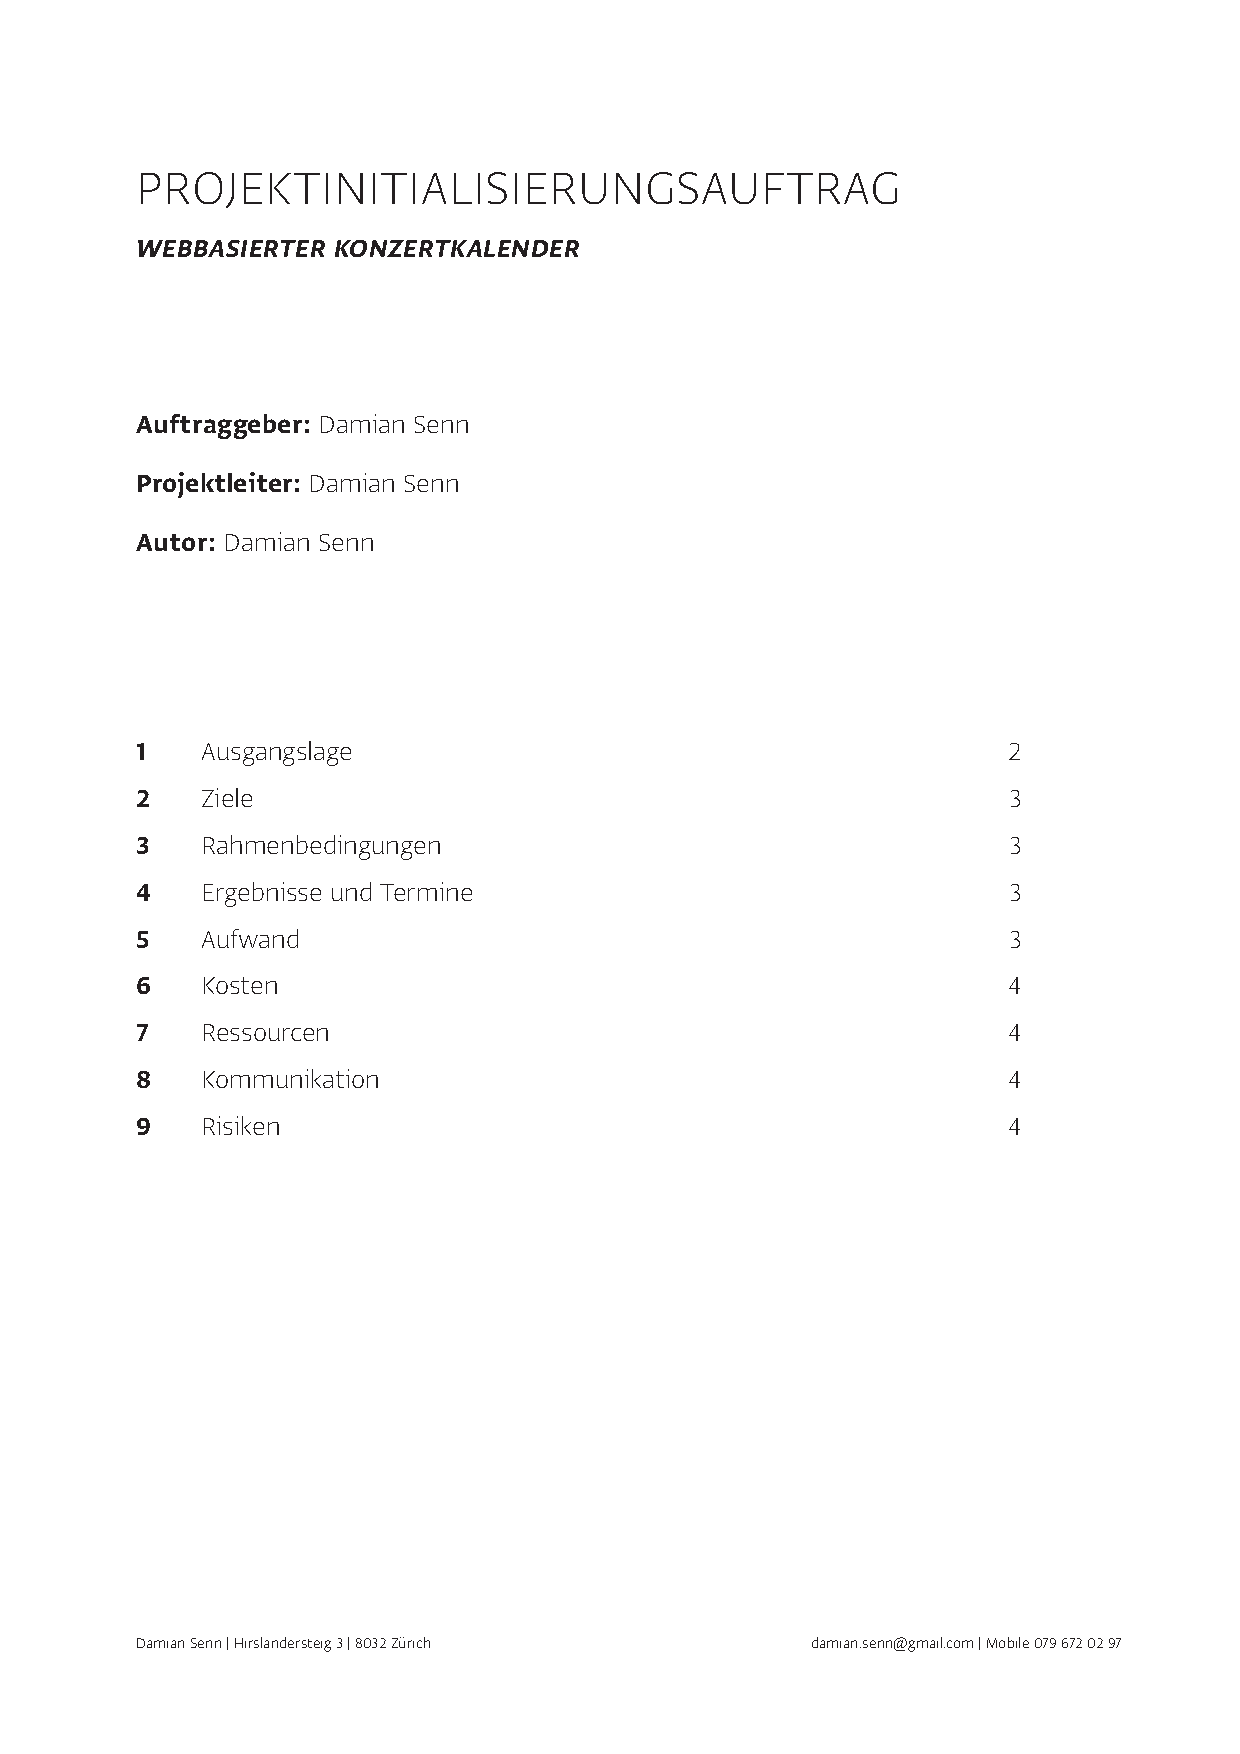
\includepdf[pages=1,pagecommand={\Hide\chapter{Projektinitialisierungsauftrag}}]{eingabe/Projektinitialisierungsauftrag.pdf}
\includepdf[pages=2-,pagecommand={}]{eingabe/Projektinitialisierungsauftrag.pdf}

\chapter{Projektauftrag}

\label{AppendixProjektauftrag}

\section{Zweck des Dokuments}\label{ProjektauftragZweck}

Der Projektauftrag ist die verbindliche Vereinbarung zwischen Auftraggeber und
Projektleiter, und bildet die Grundlage für den Projektstart sowie die
Phasenfreigaben.

Folgend sind alle wichtigen Informationen die in der Phase Initialisierung
erarbeitet wurden. Alle weiteren Details die in der Initialisierung
ausgearbeitet wurden sind in der Studie im Anhang~\ref{AppendixStudie} zu
finden.

\section{Ausgangslage}\label{ausgangslage}

Als regelmässiger Konzertbesucher wünsche ich mir eine Plattform im
Internet, auf welcher ich eine zuverlässige Übersicht an Konzerten in
meiner Umgebung vorfinde. Heute sind die Events nur verteilt auf
verschiedenen Seiten wie die der Venues, des Konzertveranstalters, des
Künstlers oder auf Facebook publiziert.\\

\noindent
Ich möchte deshalb eine zentrale Plattform entwickeln, die es Benutzern
einfach macht, Konzerte für ihren Geschmack zu finden.
Die Plattform soll Genre unabhängig sein und entsprechende Filter anbieten.
Den Benutzern der Plattform soll es möglich sein, Konzerte selber zu
erfassen und pflegen.\\

\noindent
Um einen zusätzlichen Service für den Benutzer zur Verfügungs zu stellen,
ist es auch denkbar, eine Art Notifikationssystem zu bauen um Benutzer
über Handy-Notifications oder per Email an Konzerte oder Künstler zu
erinnern.\\

\noindent
Konzertveranstaltern kann das Erfassen ihrer Events vereinfacht werden,
indem auf der Plattform erfasste Veranstaltungen direkt auf den Sozialen
Medien wie Facebook, Twitter oder Instagram geteilt werden können.


\clearpage
\section{Projektziele}\label{projektziele}

Folgende Ziele sind in der Initialisierungsphase definiert worden:

\begin{longtable}[]{@{}lll@{}}
  \toprule
  Nr.  & Zielbeschreibung                                                                       & Muss/Kann\tabularnewline
  \toprule
       & Produktziele\tabularnewline
  \midrule
  1.1  & Besucher können im Produkt nach Konzerten suchen                                       & Muss\tabularnewline
  1.2  & Suchresultate können nach Musik-Genre und Ort gefiltert werden                         & Muss\tabularnewline
  1.3  & Das Produkt soll ein modernes responsives Design vorweisen                             & Muss\tabularnewline
  1.4  & Konzerte sollen von Suchmaschinen indexiert werden können                              & Muss\tabularnewline
  1.5  & Benutzer können isch im Produkt registrieren                                           & Muss\tabularnewline
  1.6  & Benutzer können ihr Passwort nach Verlust neu setzen                                   & Muss\tabularnewline
  1.7  & Inhalte des Portals sind durch die Benutzer erfassbar und bearbeitbar                  & Muss\tabularnewline
  1.8  & Kompatibilität mit aktuellem Google Chrome und Mozilla Firefox Browser                 & Muss\tabularnewline
  1.9  & Konzerte können vom Produkt nach Facebook exportiert werden                            & Kann\tabularnewline
  1.10 & Ein angemeldeter Benutzer kann vermerken ob er einem Konzert teilnimmt                 & Kann\tabularnewline
  1.11 & Das Produkt soll sich an Security Best-Practices von OWASP halten                      & Muss\tabularnewline
  \bottomrule
       & Abwicklungsziele\tabularnewline
  \midrule
  2.1  & \makecell[l]{Das Projekt soll nach HERMES 5 unter Berücksichtigung der Richtlinien von                            \\ der TSBE dokumentiert werden} & Muss\tabularnewline
  2.2  & Das Produkt muss bis Projektende fertiggestellt und bereit für die Einführung sein     & Muss\tabularnewline
  2.3  & Die Technische-Umsetzung wird durch Damian Senn erstellt                               & Muss\tabularnewline
  2.4  & \makecell[l]{Die Kommunikation zwischen Experten und Diplomanden erfolgt wie im                                   \\ Projektauftrag \ref{kommunikation} beschrieben.} & Muss\tabularnewline
  2.5  & Das Projekt muss bis Ende Mai 2019 abgeschlossen sein                                  & Muss\tabularnewline
  \bottomrule
\end{longtable}


\section{Rahmenbedingungen}\label{rahmenbedingungen}

\begin{itemize}
  \tightlist
  \item{}
        Das Projekt wird im Rahmen der Diplomarbeit durchgeführt.
  \item{}
        Die Richtlinien zum Erstellen des Diplomberichtes der TSBE.
        müssen eingehalten werden.
  \item{}
        Als Projektmethodik wird HERMES 5 verwendet, angepasst auf das Projekt.
  \item{}
        Sämtliche Projekt-Dokumente sowie Programmcode wird regelmässig ins private Github
        Repository\footnote{\url{https://github.com/topaxi/diplomarbeit-tsbe}} geladen.
\end{itemize}

% TODO: Do I need the following?
%\clearpage
%\subsection{Begründung der
%  Projektziele}\label{begruxfcndung-der-projektziele}

\clearpage
\section{Terminplan}

Nachfolgend ist der grobe Terminplan für die geplanten Phasen. Im Anhang~\ref{terminplan} ist
der detaillierte Terminplan abgelegt.

\begin{longtable}[]{@{}lrr@{}}
  \toprule
  Phase           & Datum                   & Stunden\tabularnewline
  \midrule
  \endhead
  Initialisierung & 06.03.2019 - 31.03.2019 & 64\tabularnewline
  Konzept         & 01.04.2019 - 21.04.2019 & 66\tabularnewline
  Realisierung    & 22.04.2019 - 19.05.2019 & 136\tabularnewline
  Abschluss       & 20.05.2019 - 26.05.2019 & 36\tabularnewline
  \midrule
                  & Total:                  & 302\tabularnewline
  \bottomrule
  \caption{Terminplan}
\end{longtable}


\section{Meilensteine}\label{meilensteine}

Im Projektplan wurden folgende Meilensteine und Termine festgelegt:

\begin{longtable}[]{@{}llcl@{}}
  \toprule
  Nr. & Meilenstein                     & KW & Datum\tabularnewline
  \midrule
  \endhead
  1   & Kickoff-Meeting                 & 10 & 06.03.2019\tabularnewline
  2   & Abschluss Phase Initialisierung & 13 & 31.03.2019\tabularnewline
  3   & Zwischen-Meeting                & 18 & 24.04.2019\tabularnewline
  4   & Abschluss Phase Konzept         & 16 & 21.04.2019\tabularnewline
  5   & Abschluss Phase Realisierung    & 20 & 19.05.2019\tabularnewline
  6   & Abschluss Phase Abschluss       & 21 & \tabularnewline
  7   & Abschluss-Meeting               & 22 & \tabularnewline
  \bottomrule
  \caption{Meilensteine}
\end{longtable}

Das Datum für das Abschluss-Meeting wird im Zwischen-Meeting mit den Experten, Sandro Bertolino und Severin Räz, festgelegt. Der Abschluss der Phase Abschluss ist Abhängig vom Abschluss-Meeting und wird mindestens eine Woche vor dem Meeting stattfinden.

\clearpage

\section{Organigramm}\label{organigramm}

\begin{figure}[!htb]
  \centering
  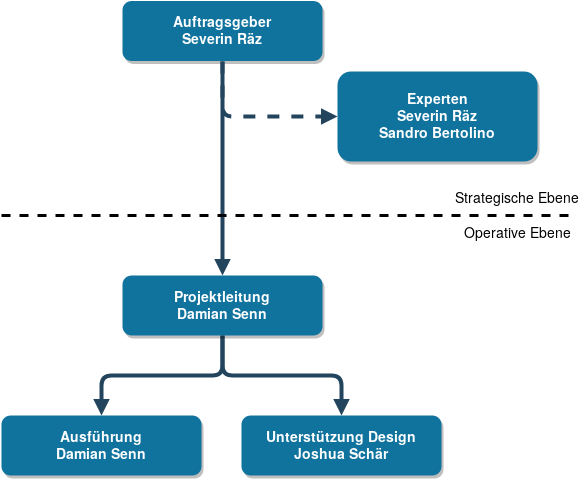
\includegraphics[width=0.8\textwidth]{figures/organigram.png}
  \caption{Organigram}
\end{figure}

\subsection{Tätigkeiten im Projekt}\label{tuxe4tigkeiten-im-projekt}

Für die Freigaben der Phasen ist nach Absprache mit Severin Räz Damian Senn
selbstständig verantwortlich.

\begin{longtable}[]{@{}ll@{}}
  \toprule
  \textbf{Name}    & \textbf{Funktions- und Tätigkeitsbereich}\tabularnewline
  \midrule
  \endhead
  Severin Räz      & Auftraggeber, externer Experte\tabularnewline
  Sandro Bertolino & Interner Experte\tabularnewline
  Damian Senn      & Projektleiter, Ausführung\tabularnewline
  Joshua Schär     & Unterstützung Design\tabularnewline
  \bottomrule
  \caption{Tätigkeiten Verteilung}
\end{longtable}

\subsection{Kommunikation}\label{kommunikation}

Wie im Kickoff-Meeting besprochen, wird Damian Senn alle zwei Wochen einen
kurzen Bericht an Sandro Bertolino und Severin Räz per E-Mail schicken.
Im Bericht wird erläutert was in der Zwischenzeit erledigt wurde und was
die nächsten Schritte im Projekt sind.

\clearpage

\section{Abgrenzungen}\label{abgrenzungen}

\begin{figure}[!htb]
  \centering
  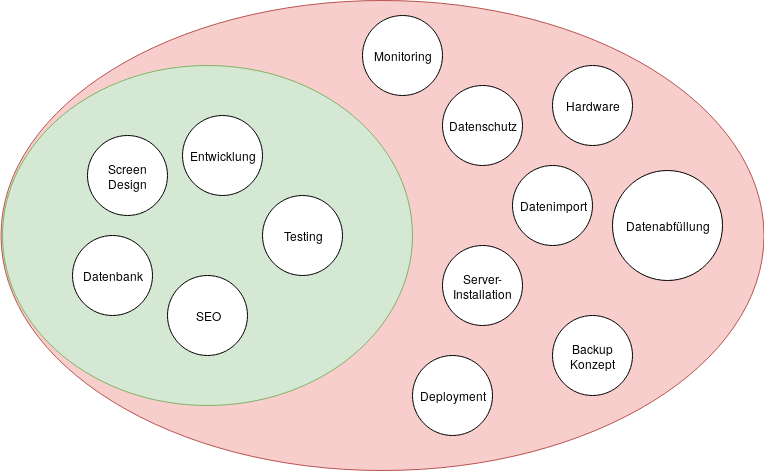
\includegraphics[width=0.95\textwidth]{figures/abgrenzungen.png}
  \caption{Abgrenzungen}
\end{figure}

\subsubsection{Hardware, Server-Installation, Deployment und
  Monitoring}\label{hardware-server-installation-deployment-und-monitoring}

Da das Projekt ein reines Software-Entwicklungs Projekt ist, werden
keine Operativen tätigkeiten wie Hardwarebeschaffung,
Server-Installation, Deployment und das einrichten eines
Monitoring-Systems vorgenommen.

\subsubsection{Datenschutz}\label{datenschutz}

Da das Projekt nicht deployed wird und somit nicht produktiv/online
gestellt wird, müssen im Rahmen dieser Projektarbeit noch keine Gedanken
über den Datenschutz gemacht werden.

\subsubsection{Datenimport}\label{datenimport}

Da wir bisher keine existierenden Konzertdaten besitzen, ist es nicht
nötig, einen Datenimport zu implementieren.

\subsubsection{Datenabfüllung}\label{datenabfuxfcllung}

Die Projektarbeit beinhaltet kein Datenset, Tests werden mit Testdaten
abgewickelt. Es liegt nicht in der Verantwortung des Projektleiters,
dass Daten in die Applikation abgefüllt werden.

\subsubsection{Backup Konzept}\label{backup-konzept}

Es wird kein Backup Konzept benötigt, da die Applikation im Rahmen
dieses Projektes nicht produktiv geschaltet wird.

\clearpage
\section{Anforderungskatalog}\label{anforderungskatalog}

Der Anforderungskatalog wurde in der Studie erarbeitet. Es wurden Kann und Muss
Kriterien definiert, wobei ein Muss-Kriterium zwingend erfüllt werden muss und
ein Kann-Kriterium als Erweiterung angesehen wird.

% TODO: Fix multirows across pages
%       https://tex.stackexchange.com/questions/79143/how-to-repeat-cell-content-on-next-page-for-longtable-using-multirow/79152
\begin{longtable}[]{@{}p{1.9cm}p{2.5cm}cp{5.5cm}cc@{}}
  \toprule
  \textbf{Feature}           & \textbf{Titel}             & \textbf{Nr.} & \textbf{Kriterium}                                                                                          & \textbf{Ziel} & \textbf{Muss}\tabularnewline
  \midrule
  \endhead
  \multirow{10}{*}{Suche}    & Suche nach Konzertname     & 1.1          & Listet alle Konzerte die Wörter der Suche im Konzertnamen beinhalten                                        & 1.1           & \textbf{Muss}                \\ \cline{2-6}
                             & Suche nach Konzertlocation & 1.2          & Schränkt die Such-Resultate nach gegebener Konzertlocation ein                                              & 1.2           & \textbf{Muss}                \\ \cline{2-6}
                             & Suche nach Ort             & 1.2          & Schränkt die Such-Resultate nach gegebenem Ort ein                                                          & 1.2           & \textbf{Muss}                \\ \cline{2-6}
                             & Suche nach Genre           & 1.2          & Schränkt die Such-Resultate nach gegebenem Musik-Genre ein                                                  & 1.2           & \textbf{Muss}                \\
  \midrule
  \multirow{8}{*}{Design}    & Desktop                    & 2.1          & Alle Ansichten haben eine Desktop-Optimierte Variante                                                       & 1.4           & \textbf{Muss}                \\ \cline{2-6}
                             & Tablet                     & 2.2          & Alle Ansichten haben eine Tablet-Optimierte Variante                                                        & 1.4           & \textbf{Muss}                \\ \cline{2-6}
                             & Mobile                     & 2.3          & Alle Ansichten haben eine Mobile-Optimierte Variante                                                        & 1.4           & \textbf{Muss}                \\ \cline{2-6}
                             & Browser Kompatibilität     & 2.4          & Alle Ansichten müssen in aktuellem Google Chrome und Mozilla Firefox dem Grundlayout folgen                 & 1.9           & \textbf{Muss}                \\
  \midrule
  \multirow{4}{*}{SEO}       & Indexierbarkeit            & 3.1          & Das Produkt ist von Suchmaschinen indexierbar                                                               & 1.5           & \textbf{Muss}                \\ \cline{2-6}
                             & Linked Data                & 3.2          & Konzert Detailseiten sind mit dem Event-Schema\footnote{\url{https://schema.org/Event}} ausgestattet              & 1.5           & \textbf{Muss}                \\
  \midrule
  \multirow{8}{*}{Benutzer}  & Registrierung              & 4.1          & Besucher können sich einen Benutzer registrieren, Benutzernamen und E-Mail Adressen müssen einzigartig sein & 1.6           & \textbf{Muss}                \\ \cline{2-6}
                             & Passwort-Vergessen         & 4.2          & Benutzer können sich einen Passwort-Reset Link anfordern                                                    & 1.7           & \textbf{Muss}                \\ \cline{2-6}
                             & Social                     & 4.3          & Benutzer können auf Konzerten vermerken ob sie Teilnehmen oder nicht                                        & 1.11          & Kann                         \\
  \midrule
  \clearpage
  \multirow{6}{*}{Erfassung} & Artist                     & 5.1          & Benutzer können Artisten mit einem Genre erfassen                                                           & 1.8           & \textbf{Muss}                \\ \cline{2-6}
                             & Location                   & 5.2          & Benutzer können eine Konzertlocation mit Ort/Strasse erfassen                                               & 1.8           & \textbf{Muss}                \\ \cline{2-6}
                             & Konzert                    & 5.3          & Benutzer können ein Konzert mit Konzertlocation und Artisten erfassen                                       & 1.8           & \textbf{Muss}                \\ \cline{2-6}
                             & Facebook                   & 5.4          & Benutzer können ein Konzert in ein Facebook-Event exportieren                                               & 1.10          & Kann                         \\
  \midrule
  \multirow{9}{*}{Security}  & SQL-Injection              & 6.1          & Das Produkt soll resistent gegen SQL-Injection sein                                                         & 1.12          & \textbf{Muss}                \\ \cline{2-6}
                             & HTML-Injection             & 6.2          & Das Produkt soll resistent gegen HTML-Injection / XSS sein                                                  & 1.12          & \textbf{Muss}                \\ \cline{2-6}
                             & Passwort encryption        & 6.3          & Passwörter von Benutzer müssen mit einem sicheren Verfahren gespeichert werden                              & 1.12          & \textbf{Muss}                \\ \cline{2-6}
                             & Session                    & 6.4          & Session-Cookies dürfen nicht durch JavaScript ausgelesen werden                                             & 1.12          & Kann                         \\
  \midrule
  Performance                & Ladezeit                   & 7.1          & Die Seitenansichten dürfen nicht länger als 6 Sekunden auf einem 3G Netz laden                              &               & \textbf{Muss}                \\
  \midrule
  Sonstiges                  & User Tracking              & 8.1          & Benutzerverhalten soll analysiert und nachvollziehbar sein.                                                 &               & Kann                         \\
  \bottomrule
  \caption{Anforderungskatalog}
\end{longtable}


\clearpage
\section{Lösungsbeschreibung}\label{loesungsbeschreibung}

In der Studie (Anhang~\ref{AppendixStudie}) wurden Technologien gegenüber
gestellt und für die Umsetzung mittels Nutzwertanalysen ausgewählt.\\

\noindent
Folgende Technologien wurden ausgewählt:\\

\textbf{Browser sowie Server Technologie:}

\begin{figure}[!htb]
  \centering
  
\includegraphics[width=0.8\textwidth]{figures/phoenix.png}
  \captionsource{Phoenix Framework Logo}{\url{https://github.com/phoenixframework/phoenix}}
\end{figure}

\noindent
Die Nutzwertanalyse hat ergeben, dass es sinnvoller ist, das Projekt mit
einer klassischen SSR Applikation zu starten. Das Phoenix Framework bietet alle
benötigten Features an und kann durch zusätzliche Module einfach erweitert werden.

Für dynamische Interaktionen wie Formular-Validierungen wird zu einfachem
JavaScript gegriffen. Ist ein Screen besonders interaktiv, kann gegebenenfalls
eine kleinere JavaScript-Library verwendet werden um die Problemlösung zu
vereinfachen.\\

\textbf{Testing Technologie:}

\begin{figure}[!htb]
  \centering
  
\includegraphics[width=0.8\textwidth]{figures/wallaby.png}
  \captionsource{Wallaby Logo}{\url{https://github.com/keathley/wallaby}}
\end{figure}

\noindent
Getestet wird die Applikation durch die von Phoenix gegebenen Testing-Tools
sowie mit der Browser-Testing Library «Wallaby».

\clearpage
\section{Kosten}\label{projektauftragkosten}

In der Studie wurden die Projekt- sowie Betriebskosten ausgerechnet.

Der gesamte Personalaufwand beträgt \textbf{42'900} für die geplanten Stunden.

\begin{longtable}[]{@{}lrr@{}}
  \toprule
  \textbf{Phase}  & \makecell[r]{\textbf{Geplante} \\\textbf{Stunden}} & \textbf{Kosten}\tabularnewline
  \midrule
  \endhead
  Initialisierung &  64                       &  9'600.- CHF\tabularnewline
  Konzept         &  66                       &  9'900.- CHF\tabularnewline
  Realisierung    & 136                       & 20'400.- CHF\tabularnewline
  Abschluss       &  64                       &  5'400.- CHF\tabularnewline
  \midrule
  \textbf{Total:} & 286                       & 42'900.- CHF\tabularnewline
  \bottomrule
  \caption{Projektkosten}
\end{longtable}


Für die Betriebskosten wurde angenommen, dass das Produkt in der Cloud auf
einer mittelgrossen Umgebung betrieben wird. Die Kosten dieser Umgebung wurde
auf 150.- CHF pro Monat geschätzt.

Neben der Umgebung muss mindestens eine Domain gekauft und jährlich bezahlt
werden. Die Kosten einer Domain sind rund 20.- CHF pro Jahr.

Da jediglich Open Source Software eingesetzt wird, gibt es keine
Software-Lizenzen zu bezahlen.

\begin{longtable}[]{@{}lll@{}}
  \toprule
  \textbf{Kostenstelle} & \textbf{Jährliche Kosten}\tabularnewline
  \midrule
  \endhead
  Software              & Keine\tabularnewline
  .com Domain           & 20.- CHF\tabularnewline
  Hosting               & 1'800.- CHF\tabularnewline
  \midrule
  \textbf{Total:}       & 1'820.- CHF\tabularnewline
  \bottomrule
  \caption{Betriebskosten}
\end{longtable}


\clearpage
\section{Risiken}\label{risiken}

Die Risikobewertung erfolgt mit folgender Formel:\\

\textbf{Bewertung = Schaden x Eintrittswahrscheinlichkeit}\\

\noindent
Schadensskala:

\begin{longtable}[]{@{}lp{11cm}@{}}
  \toprule
  \textbf{Gewichtung} & \textbf{Beschreibung}\tabularnewline
  \midrule
  \endhead
  Gering (1-2)        & Kleiner Schaden, hat kaum Auswirkungen auf das Projekt.\tabularnewline
  Mittel (3-4)        & Mittlerer Schaden, Zeitverzögerungen oder Qualitätsverluste.\tabularnewline
  Hoch (5-6)          & Hoher Schaden, wichtige Arbeiten oder Phasen können nicht abgeschlossen werden, schlimmstenfalls ein Abbruch des Projekts.\tabularnewline
  \bottomrule
  \caption{Risiken - Schadensskala}
\end{longtable}

\noindent
Eintrittswahrscheinlichkeitsskala:

\begin{longtable}[]{@{}lp{12cm}@{}}
  \toprule
  \textbf{Gewichtung} & \textbf{Beschreibung}\tabularnewline
  \midrule
  \endhead
  Gering (1-2)        & Kleine Eintrittswahrscheinlichkeit.\tabularnewline
  Mittel (3-4)        & Mittlere Eintrittswahrscheinlichkeit.\tabularnewline
  Hoch (5-6)          & Hohe Eintrittswahrscheinlichkeit.\tabularnewline
  \bottomrule
  \caption{Risiken - Eintrittswahrscheinlichkeit}
\end{longtable}

\noindent
Handlungen um Risikobewertungen zu senken:

\begin{longtable}[]{@{}lp{12cm}@{}}
  \toprule
  \textbf{Handlung} & \textbf{Beschreibung}\tabularnewline
  \midrule
  \endhead
  Akzeptanz         & Das Eintreten eines Risiko wird wissentlich angenommen.\tabularnewline
  Transfer          & Die Verantwortung von Risiken können an Dritte abgegeben werden.\tabularnewline
  Verminderung      & Der Schaden oder die Eintrittswahrscheinlichkeit kann begrenzt oder reduziert werden.\tabularnewline
  Vermeidung        & Es kann jeglichen Schaden vermieden werden.\tabularnewline
  \bottomrule
  \caption{Risiken - Handlungen zur Senkung der Bewertung}
\end{longtable}


\clearpage
\subsection{Projektrisiken}\label{projektrisiken}

\begin{longtable}[]{@{}lp{3cm}p{4cm}ccc@{}}
  \toprule
  \textbf{Nr.} & \textbf{Risiko}                             & \textbf{Auswirkung}                                 & \textbf{Schaden} & \textbf{Wahrsch.} & \textbf{Bewertung}\tabularnewline
  \midrule
  \endhead
  1            & Ausfall des Entwicklers oder Projektleiters & Verzögerungen von Arbeiten                          & 4                & 3                 & Mittel\tabularnewline
  2            & Unvollständige Projektdokumentation         & Schlechtere Diplomarbeit Bewertung                  & 4                & 2                 & Mittel\tabularnewline
  3            & Schlechter Projektplan                      & Verzögerungen und eventuelle Qualitätsverluste      & 4                & 3                 & Mittel\tabularnewline
  4            & Keine Benutzer                              & Das Produkt wird nicht von Benutzern eingesetzt     & 3                & 4                 & Mittel\tabularnewline
  5            & Technisch nicht umsetzbare Features         & Das Produkt kann nicht wie angedacht benutzt werden & 4                & 3                 & Mittel\tabularnewline
  \bottomrule
  \caption{Projektrisiken}
\end{longtable}

\clearpage
\subsection{Massnahmen}\label{massnahmen}

\begin{longtable}[]{@{}lp{4.1cm}lccc@{}}
  \toprule
               &                                                                       &                   & \multicolumn{3}{l}{\textbf{Bewertung nach Massnahme}}\tabularnewline
  \textbf{Nr.} & \textbf{Massnahme}                                                    & \textbf{Handlung} & \textbf{Schaden}                                                     & \textbf{Wahrsch.} & \textbf{Bewertung}\tabularnewline
  \midrule
  \endhead
  1            & Arzt aufsuchen, ggf. Projekt-Pause oder Abbruch                       & Akzeptanz         & 4                                                                    & 3                 & Mittel\tabularnewline
  2            & Statusbericht alle zwei Wochen, bei Fragen sofort Hilfe suchen        & Verminderung      & 2                                                                    & 1                 & Gering\tabularnewline
  3            & Genügend Buffer-Zeit einplanen, ggf. Ferientage für Projekt einsetzen & Verminderung      & 2                                                                    & 1                 & Gering\tabularnewline
  4            & Das Produkt löst vor allem ein persönliches Interesse                 & Akzeptanz         & 3                                                                    & 4                 & Mittel\tabularnewline
  5            & Vereinfachte Alternativen in Konzept-Phase untersuchen                & Verminderung      & 2                                                                    & 2                 & Gering\tabularnewline
  \bottomrule
  \caption{Projektrisiken - Massnahmen}
\end{longtable}

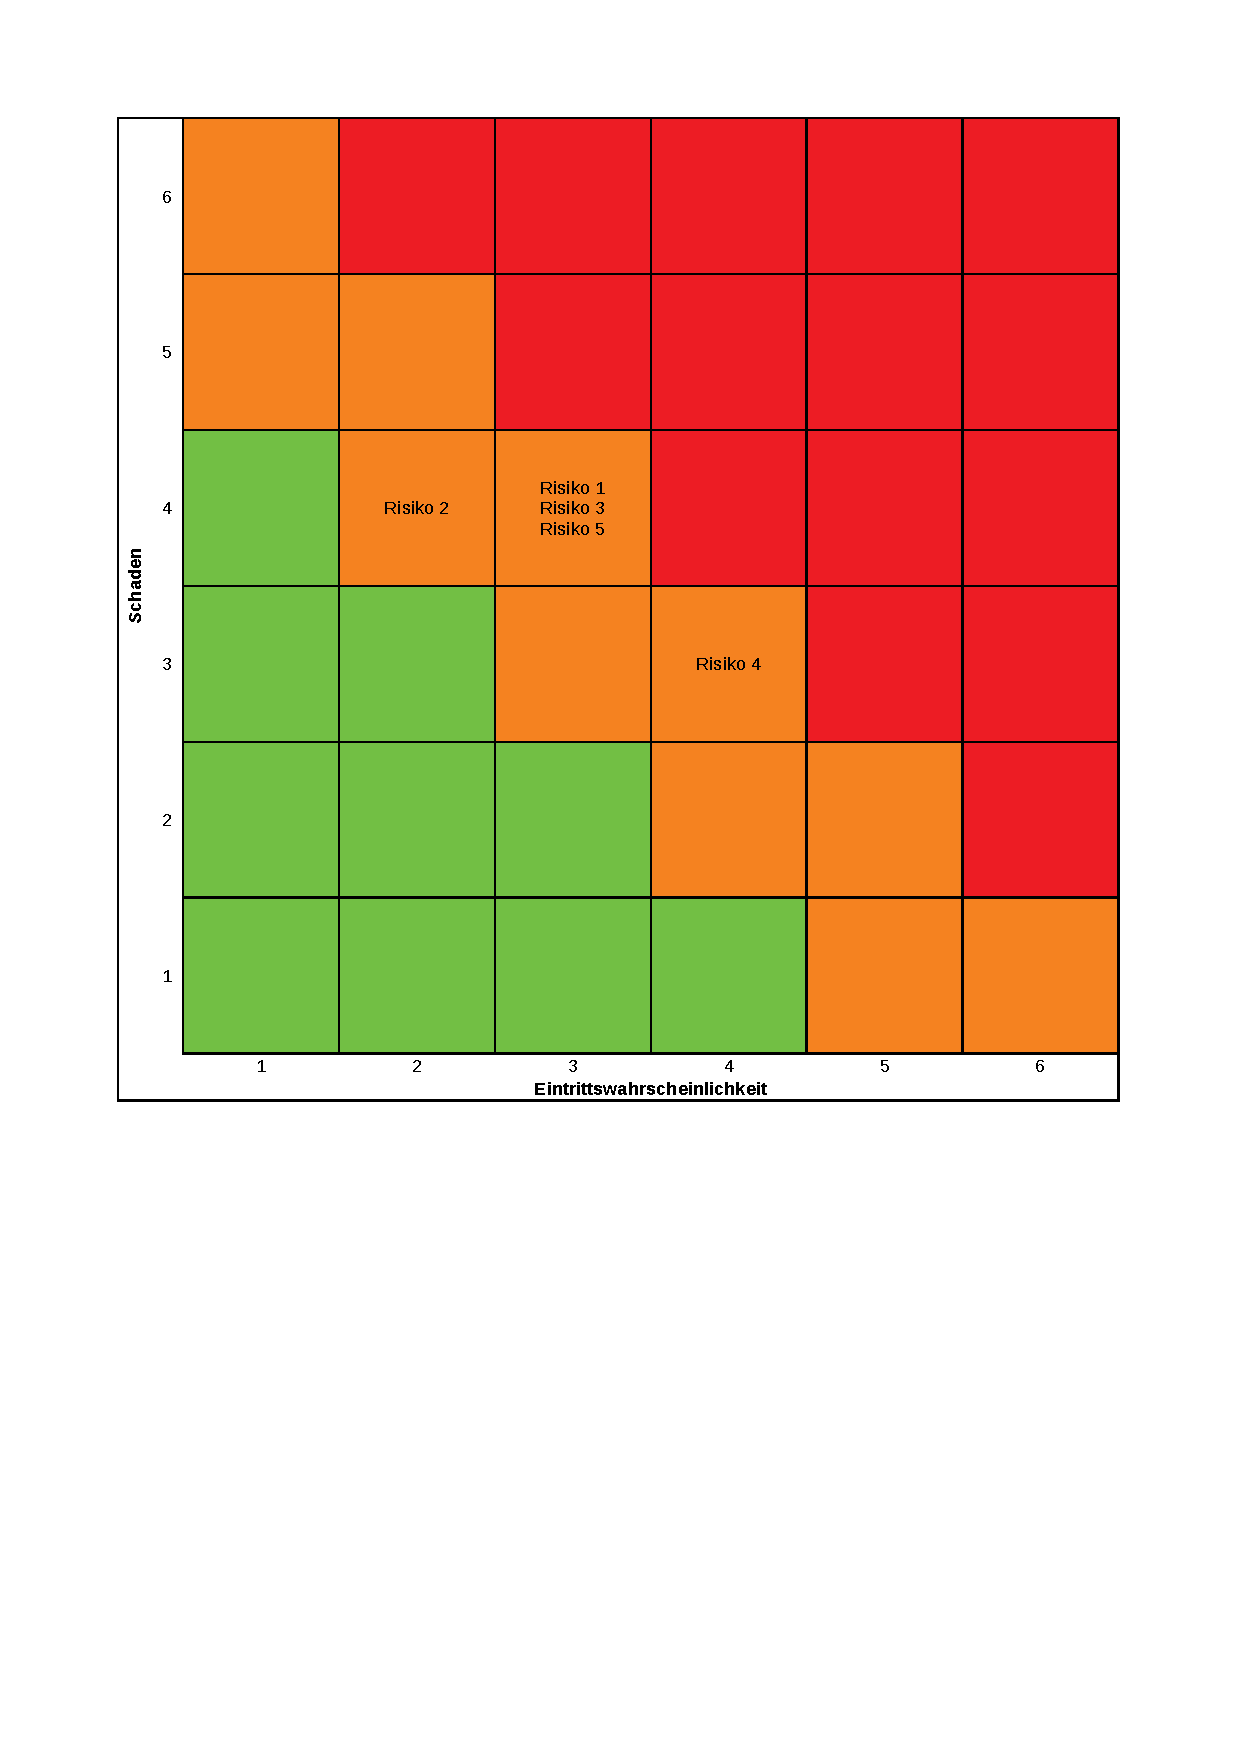
\includepdf[pages=1, pagecommand={\subsection{Risikodiagramm ohne Massnahmen}\label{risikodiagram-ohne-massnahmen}}, trim=0mm 80mm 0mm 0mm, clip]{initialisierung/risiko.pdf}
\includepdf[pages=2, pagecommand={\subsection{Risikodiagramm mit Massnahmen}\label{risikodiagram-mit-massnahmen}}, trim=0mm 80mm 0mm 0mm, clip]{initialisierung/risiko.pdf}

\chapter{Studie}

\label{AppendixStudie}

\section{Zweck des Dokuments}\label{StudieZweck}

In der Studie werden die Anforderungen aufgenommen, sowie Variantenbeschriebe
für die Projektrealisierung erstellt. Die Varianten werden miteinander
verglichen und durch den Variantenentscheid wird das weitere
Vorgehen definiert.
Ausserdem werden in der Studie die Risiken und Wirtschaftlichkeit des Projekts
analysiert.

Folgende Arbeiten werden in dieser Studie abgehandelt:

\begin{itemize}
  \tightlist
  \item der Anforderungskatalog wird definiert
  \item die Evaluation der Browser Software-Technologien
  \item die Evaluation der Server Software-Technologien
  \item die Evaluation der Testing Software-Technologien
  \item eine Kostenschätzung und mögliche Wirtschaftlichkeit ausgerechnet
\end{itemize}


\section{Informationsbeschaffung}\label{informationsbeschaffung}

\begin{longtable}[]{@{}lp{10cm}@{}}
  \toprule
  Quelle                        & Beschreibung\tabularnewline
  \toprule
  Schulwissen / Berufserfahrung & Die Grundlage für die Umsetzung dieses Projekts wird durch mein existierendes Schulwissen sowie meine langjährige Berufserfahrung in der Software-Entwicklung gesetzt.\tabularnewline
  \midrule
  Internet                      & Ein Grossteil der Informationen werden heute über das Internet bezogen, für die Evaluation von Technologien und Lösungsansätzen wird einiges über das Internet recherchiert werden müssen.\tabularnewline
  \bottomrule
  \caption{Informationsbeschaffung}
\end{longtable}

\clearpage
\section{Anforderungskatalog}\label{anforderungskatalog}

% TODO: Fix multirows across pages
%       https://tex.stackexchange.com/questions/79143/how-to-repeat-cell-content-on-next-page-for-longtable-using-multirow/79152
\begin{longtable}[]{@{}p{1.9cm}p{2.5cm}cp{5.5cm}cc@{}}
  \toprule
  \textbf{Feature}           & \textbf{Titel}             & \textbf{Nr.} & \textbf{Kriterium}                                                                                          & \textbf{Ziel} & \textbf{Muss}\tabularnewline
  \midrule
  \endhead
  \multirow{10}{*}{Suche}    & Suche nach Konzertname     & 1.1          & Listet alle Konzerte die Wörter der Suche im Konzertnamen beinhalten                                        & 1.1           & \textbf{Muss}                \\ \cline{2-6}
                             & Suche nach Konzertlocation & 1.2          & Schränkt die Such-Resultate nach gegebener Konzertlocation ein                                              & 1.2           & \textbf{Muss}                \\ \cline{2-6}
                             & Suche nach Ort             & 1.2          & Schränkt die Such-Resultate nach gegebenem Ort ein                                                          & 1.2           & \textbf{Muss}                \\ \cline{2-6}
                             & Suche nach Genre           & 1.2          & Schränkt die Such-Resultate nach gegebenem Musik-Genre ein                                                  & 1.2           & \textbf{Muss}                \\
  \midrule
  \multirow{8}{*}{Design}    & Desktop                    & 2.1          & Alle Ansichten haben eine Desktop-Optimierte Variante                                                       & 1.4           & \textbf{Muss}                \\ \cline{2-6}
                             & Tablet                     & 2.2          & Alle Ansichten haben eine Tablet-Optimierte Variante                                                        & 1.4           & \textbf{Muss}                \\ \cline{2-6}
                             & Mobile                     & 2.3          & Alle Ansichten haben eine Mobile-Optimierte Variante                                                        & 1.4           & \textbf{Muss}                \\ \cline{2-6}
                             & Browser Kompatibilität     & 2.4          & Alle Ansichten müssen in aktuellem Google Chrome und Mozilla Firefox dem Grundlayout folgen                 & 1.9           & \textbf{Muss}                \\
  \midrule
  \multirow{4}{*}{SEO}       & Indexierbarkeit            & 3.1          & Das Produkt ist von Suchmaschinen indexierbar                                                               & 1.5           & \textbf{Muss}                \\ \cline{2-6}
                             & Linked Data                & 3.2          & Konzert Detailseiten sind mit dem Event-Schema\footnote{\url{https://schema.org/Event}} ausgestattet              & 1.5           & \textbf{Muss}                \\
  \midrule
  \multirow{8}{*}{Benutzer}  & Registrierung              & 4.1          & Besucher können sich einen Benutzer registrieren, Benutzernamen und E-Mail Adressen müssen einzigartig sein & 1.6           & \textbf{Muss}                \\ \cline{2-6}
                             & Passwort-Vergessen         & 4.2          & Benutzer können sich einen Passwort-Reset Link anfordern                                                    & 1.7           & \textbf{Muss}                \\ \cline{2-6}
                             & Social                     & 4.3          & Benutzer können auf Konzerten vermerken ob sie Teilnehmen oder nicht                                        & 1.11          & Kann                         \\
  \midrule
  \clearpage
  \multirow{6}{*}{Erfassung} & Artist                     & 5.1          & Benutzer können Artisten mit einem Genre erfassen                                                           & 1.8           & \textbf{Muss}                \\ \cline{2-6}
                             & Location                   & 5.2          & Benutzer können eine Konzertlocation mit Ort/Strasse erfassen                                               & 1.8           & \textbf{Muss}                \\ \cline{2-6}
                             & Konzert                    & 5.3          & Benutzer können ein Konzert mit Konzertlocation und Artisten erfassen                                       & 1.8           & \textbf{Muss}                \\ \cline{2-6}
                             & Facebook                   & 5.4          & Benutzer können ein Konzert in ein Facebook-Event exportieren                                               & 1.10          & Kann                         \\
  \midrule
  \multirow{9}{*}{Security}  & SQL-Injection              & 6.1          & Das Produkt soll resistent gegen SQL-Injection sein                                                         & 1.12          & \textbf{Muss}                \\ \cline{2-6}
                             & HTML-Injection             & 6.2          & Das Produkt soll resistent gegen HTML-Injection / XSS sein                                                  & 1.12          & \textbf{Muss}                \\ \cline{2-6}
                             & Passwort encryption        & 6.3          & Passwörter von Benutzer müssen mit einem sicheren Verfahren gespeichert werden                              & 1.12          & \textbf{Muss}                \\ \cline{2-6}
                             & Session                    & 6.4          & Session-Cookies dürfen nicht durch JavaScript ausgelesen werden                                             & 1.12          & Kann                         \\
  \midrule
  Performance                & Ladezeit                   & 7.1          & Die Seitenansichten dürfen nicht länger als 6 Sekunden auf einem 3G Netz laden                              &               & \textbf{Muss}                \\
  \midrule
  Sonstiges                  & User Tracking              & 8.1          & Benutzerverhalten soll analysiert und nachvollziehbar sein.                                                 &               & Kann                         \\
  \bottomrule
  \caption{Anforderungskatalog}
\end{longtable}


\clearpage
\section{Evaluation Browser-Technologie}\label{evaluation-browser-technologie}

\begin{longtable}[]{@{}p{2cm}cp{10cm}@{}}
  \toprule
  \textbf{Kriterium} & \textbf{Gewicht} & \textbf{Abnahmekriterium}\tabularnewline
  \midrule
  \endhead
  Komplexität        & 3                & Die Technologie sollte im Rahmen der Diplomarbeit nicht eine zu hohe Komplexität vorweisen. Durch eine niedrigere Komplexität bestehen weniger Risiken dass technische Probleme auftreten werden.\tabularnewline
  \midrule
  Performance        & 4                & In den Projektzielen wurde definiert, dass die Applikation in maximal 6 Sekunden im Browser geladen sein muss. Daher ist es wichtig, dass die Technologie gute Performance Charakteristiken vorweist.\tabularnewline
  \midrule
  SEO                & 5                & Für eine öffentliche Applikation ist es unentbehrlich, dass sie indexierbar durch Suchmaschinen ist.\tabularnewline
  \midrule
  Interaktivität     & 4                & Applikationen im Browser werden immer interaktiver, daher ist es wichtig, das die Technologie anspruchsvolle Abläufe implementieren kann. \tabularnewline
  \midrule
  Stabilität         & 3                & Für das Projekt ist es wichtig, dass auf eine stabile Technologie gesetzt wird, welche den Projektablauf so wenig wie möglich beeinträchtigt. \tabularnewline
  \midrule
  Testing            & 3                & Durch einfaches Testing, kann sichergestellt werden, dass die Applikation wie gewünscht umgesetzt wurde und auch beim Weiterentwickeln nicht existierende Funktionalitäten beinträchtigt werden.\tabularnewline
  \bottomrule
  \caption{Browser-Technologie Kriterien}
\end{longtable}

\subsection{Variante: React}

Die JavaScript Library \textbf{React} ist heute die wohl beliebteste
Technologie um interaktive Applikationen im Web zu bauen.

\subsection{Variante: Next.js}

\textbf{Next.js} ist ein JavaScript Framework, das auf der \textbf{React}
Library aufbaut und zusätzliche Features sowie gängige Konventionen mitbringt.

\subsection{Variante: SSR}

\textbf{SSR} steht für \textbf{S}erver\textbf{s}ide \textbf{R}endering und
beschreibt die klassische Methode vom Erstellen von Webseiten, indem man HTML
auf dem Server generiert und zum Browser schickt.

Dies hat nach wie vor seine Daseinsberechtigung, da dies weniger Komplexität
mit sich bringt, einen schnelleren Seitenaufbau garantiert und ohne
zusätzlichen Aufwand von Suchmaschinen indexiert wird.

\clearpage
\section{Bewertungen Browser-Technologie}\label{bewertungen-browser-technologie}

\textbf{Bewertung:}\\
\textit{4 = Sehr gut, 3 = Gut, 2 = Ungenügend, 1 = Schlecht}\\
\textbf{Gewichtung:}\\
\textit{5 = Unverzichtbar, 4 = Sehr wichtig, 3 = Erleichtert die Arbeit, 2 = Weniger wichtig, 1 = unwichtig}\\

\textbf{\textit{Bewertung x Gewichtung = Punktzahl}}

\begin{longtable}[]{@{}p{2cm}ccccccc@{}}
  \toprule
  \textbf{Kriterium} & \textbf{Gewichtung} & \multicolumn{2}{c}{\textbf{Variante: React}} & \multicolumn{2}{c}{\textbf{Variante: Next.js}} & \multicolumn{2}{c}{\textbf{Variante: SSR}}\tabularnewline
                     &                     & Bewertung                                    & Punkte                                         & Bewertung                                                 & Punkte & Bewertung & Punkte \tabularnewline
  \midrule
  \endhead
  Komplexität        & 3                   & 2                                            & 6                                              & 3                                                         & 9      & 4         & 12 \tabularnewline
  Performance        & 4                   & 3                                            & 12                                             & 3                                                         & 12     & 4         & 16 \tabularnewline
  SEO                & 5                   & 2                                            & 10                                             & 4                                                         & 20     & 4         & 20 \tabularnewline
  Interaktivität     & 4                   & 4                                            & 16                                             & 4                                                         & 16     & 3         & 12 \tabularnewline
  Stabilität         & 3                   & 2                                            & 6                                              & 3                                                         & 9      & 4         & 12 \tabularnewline
  Testing            & 4                   & 4                                            & 16                                             & 4                                                         & 16     & 4         & 16 \tabularnewline
  \midrule
  \textbf{Total:}    &                     & React:                                       & 66                                             & Next.js:                                                  & 82     & SSR:      & 88 \tabularnewline
  \bottomrule
  \caption{Browser-Technologie Bewertung}
\end{longtable}

\section{Entscheid Browser-Technologie}\label{entscheid-browser-technologie}

Durch die Evaluierung wurde klar, dass das Einsetzen eines JavaScript-Frameworks
zuviel zusätzliche Komplexität und gewisse einbussungen in Performance und Stabilität
unvermeidbar ist. Somit ist ein die Wahl für eine klassische Server-Side Rendered
Webseite favorisierend.

Es ist durchaus vorstellbar, dass in einem zweiten Schritt, nach diesem Projekt,
die Server-Side Rendered Applikation durch eine Next.js Applikation ersetzt werden
könnte.

\clearpage
\section{Evaluation Server-Technologie}\label{evaluation-server-technologie}

\begin{longtable}[]{@{}p{2cm}cp{10cm}@{}}
  \toprule
  \textbf{Kriterium} & \textbf{Gewicht} & \textbf{Abnahmekriterium}\tabularnewline
  \midrule
  \endhead
  Komplexität        & 3                & Die Technologie sollte im Rahmen der Diplomarbeit nicht eine zu hohe Komplexität vorweisen. Durch eine niedrigere Komplexität bestehen weniger Risiken dass technische Probleme auftreten werden.\tabularnewline
  \midrule
  Performance        & 4                & In den Projektzielen wurde definiert, dass die Applikation in maximal 6 Sekunden im Browser geladen sein muss. Daher ist es wichtig, dass die Technologie gute Performance Charakteristiken vorweist.\tabularnewline
  \midrule
  Stabilität         & 5                & Während es für die Browser-Technologie vorstellbar ist, die Technologie auszuwechseln, ist es für den Server wichtig auf eine stabile und zukunftssichere Technologie zu setzen.\tabularnewline
  \midrule
  Testing            & 5                & Durch einfaches Testing, kann sichergestellt werden, dass die Applikation wie gewünscht umgesetzt wurde und auch beim Weiterentwickeln nicht existierende Funktionalitäten beinträchtigt werden. Vorallem auf dem Server ist wichtig, dass die Businesslogik gut abdeckend gestestet werden kann.\tabularnewline
  \bottomrule
  \caption{Server-Technologie Kriterien}
\end{longtable}

\subsection{Variante: Node.js / koa.js}

Auch auf dem Server gewinnt JavaScript immer mehr an Beliebtheit.
Mit Node.js und koa.js können schnell kleinere und simplere Applikationen
erstellt werden, die dennoch sehr performant sind.

\subsection{Variante: Elixir / Phoenix}

Elixir ist eine Programmiersprache die eine sehr stabile und performante Grundlage
bietet. Durch das Framework Phoenix, wird im Elixir Ökosystem ein starkes feature
umfangreiches Web-Framework angeboten.

\subsection{Variante: Next.js}

Next.js wurde bereits als Variante für die Browser-Technologie in Betracht
gezogen. Ein zusätzliches Feature von Next.js ist, dass die Applikation auch
auf dem Server betrieben werden kann.
Das Einsetzen der selben Technologie kann bedeutende Vorteile mit sich bringen,
so muss man nur ein Framework lernen und kann Programmcode auf dem Server mit
der Applikation im Browser geteilt werden.

\clearpage
\section{Bewertungen Server-Technologie}\label{bewertungen-server-technologie}

\textbf{Bewertung:}\\
\textit{4 = Sehr gut, 3 = Gut, 2 = Ungenügend, 1 = Schlecht}\\
\textbf{Gewichtung:}\\
\textit{5 = Unverzichtbar, 4 = Sehr wichtig, 3 = Erleichtert die Arbeit, 2 = Weniger wichtig, 1 = unwichtig}\\

\textbf{\textit{Bewertung x Gewichtung = Punktzahl}}

\begin{longtable}[]{@{}p{2cm}ccccccc@{}}
  \toprule
  \textbf{Kriterium} & \textbf{Gewichtung} & \multicolumn{2}{c}{\textbf{Variante: koa.js}} & \multicolumn{2}{c}{\textbf{Variante: Phoenix}} & \multicolumn{2}{c}{\textbf{Variante: Next.js}}\tabularnewline
                     &                     & Bewertung                                     & Punkte                                         & Bewertung                                                     & Punkte & Bewertung & Punkte \tabularnewline
  \midrule
  \endhead
  Komplexität        & 3                   & 2                                             & 6                                              & 4                                                             & 12     & 3         & 9 \tabularnewline
  Performance        & 4                   & 4                                             & 16                                             & 4                                                             & 16     & 3         & 12 \tabularnewline
  Stabilität         & 5                   & 3                                             & 15                                             & 4                                                             & 20     & 3         & 15 \tabularnewline
  Testing            & 5                   & 3                                             & 15                                             & 4                                                             & 20     & 4         & 20 \tabularnewline
  \midrule
  \textbf{Total:}    &                     & koa.js:                                       & 55                                             & Phoenix:                                                      & 68     & Next.js:  & 56 \tabularnewline
  \bottomrule
  \caption{Server-Technologie Bewertung}
\end{longtable}

\section{Entscheid Server-Technologie}\label{entscheid-server-technologie}

Durch das grosse Featureste von Phoenix sowie tiefer Komplexität gegenüber den
beiden anderen Varianten hat sich Phoenix für die Server-Technologie ganz klar
durchgesetzt.

\clearpage
\section{Evaluation Testing-Technologie}\label{evaluation-testing-technologie}

\begin{longtable}[]{@{}p{2cm}cp{10cm}@{}}
  \toprule
  \textbf{Kriterium}  & \textbf{Gewicht} & \textbf{Abnahmekriterium}\tabularnewline
  \midrule
  \endhead
  Performance         & 3                & Bei wachsender Anzahl von Tests ist es wichtig, dass die Test-Software genug skalierbar ist um Tests in parallel auszuführen.\tabularnewline
  \midrule
  Stabilität          & 5                & \tabularnewline
  \midrule
  Backend-Integration & 4                & Es ist sehr hilfreich, wenn die End-to-End Test-Software vom Server direkt ausgeführt werden. So kann gleichzeitig zum Browser-Test auch die Businesslogik getestet werden.\tabularnewline
  \midrule
  Visualtesting       & 5                & Die Technologie soll mit dem Service percy.io integrierbar sein.\tabularnewline
  \bottomrule
  \caption{Testing-Technologie Kriterien}
\end{longtable}

\subsection{Jest + Puppeteer}

Jest ist ein JavaScript-Test Framework von Facebook. Durch die Kombinierung der
Puppeteer Library von Google ist es möglich, automatisierte Browser-Tests
durchzuführen.

\subsection{Wallaby}

Wallaby ist ein Elixir Browser-Test Framework, welches sich nahtlos mit Phoenix
integrieren lässt. Wallaby unterstützt parallelisierung von Tests und ist daher
ein guter Kanditat eine hohe Anzahl von automatisierten Tests.

\clearpage
\section{Bewertungen Testing-Technologie}\label{bewertungen-testing-technologie}

\textbf{Bewertung:}\\
\textit{4 = Sehr gut, 3 = Gut, 2 = Ungenügend, 1 = Schlecht}\\
\textbf{Gewichtung:}\\
\textit{5 = Unverzichtbar, 4 = Sehr wichtig, 3 = Erleichtert die Arbeit, 2 = Weniger wichtig, 1 = unwichtig}\\

\textbf{\textit{Bewertung x Gewichtung = Punktzahl}}

\begin{longtable}[]{@{}p{2cm}ccccc@{}}
  \toprule
  \textbf{Kriterium}  & \textbf{Gewichtung} & \multicolumn{2}{c}{\textbf{Variante: Jest}} & \multicolumn{2}{c}{\textbf{Variante: Wallaby}}\tabularnewline
                      &                     & Bewertung                                   & Punkte                                                        & Bewertung & Punkte\tabularnewline
  \midrule
  \endhead
  Performance         & 3                   & 4                                           & 12                                                            & 4         & 12\tabularnewline
  Stabilität          & 5                   & 3                                           & 15                                                            & 4         & 20\tabularnewline
  Backend-Integration & 4                   & 2                                           & 8                                                             & 4         & 16\tabularnewline
  Visualtesting       & 4                   & 4                                           & 16                                                            & 1         & 4\tabularnewline
  \midrule
  \textbf{Total:}     &                     & Jest:                                       & 51                                                            & Wallaby:  & 52\tabularnewline
  \bottomrule
  \caption{Testing-Technologie Bewertung}
\end{longtable}

\section{Entscheid Testing-Technologie}\label{entscheid-testing-technologie}

Dadurch dass sich Wallaby einfach mit der ausgewählten Server-Technologie
verwenden lässt, hohe Performance und Stabilität aufweist, ist Wallaby die
knapp bessere Variante als eine Jest + Puppeteer kombination.

Leider hat Wallaby keine Visualtesting Integration mit dem Dienst percy.io,
dies könnte aber im verlaufe der Umsetzung eventuell im Rahmen dieser Arbeit
umgesetzt werden.

\clearpage
\section{Wirtschaftlichkeit}\label{wirtschaftlichkeit}

\subsection{Projektkosten}

Für die Berechnung der Projektkosten wird ein Stundensatz von 150.- CHF angenommen.

\begin{longtable}[]{@{}lll@{}}
  \toprule
  \textbf{Phase}  & \textbf{Geplante Stunden} & \textbf{Kosten}\tabularnewline
  \midrule
  \endhead
  Initialisierung & 64                        & 9'600.- CHF\tabularnewline
  Konzept         & 66                        & 9'900.- CHF\tabularnewline
  Realisierung    & 136                       & 20'400.- CHF\tabularnewline
  Initialisierung & 64                        & 5'400.- CHF\tabularnewline
  \midrule
  \textbf{Total:} & 286                       & 42'900.- CHF\tabularnewline
  \bottomrule
  \caption{Projektkosten}
\end{longtable}

\noindent
Die geplanten Projektkosten betragen somit \textbf{42'900.- CHF}.

\begin{longtable}[]{@{}lll@{}}
  \toprule
  \textbf{Kostenstelle} & \textbf{Jährliche Kosten}\tabularnewline
  \midrule
  \endhead
  .com Domain           & 20.- CHF\tabularnewline
  Hosting               & 1'800.- CHF\tabularnewline
  \midrule
  \textbf{Total:}       & 1'820.- CHF\tabularnewline
  \bottomrule
  \caption{Betriebskosten}
\end{longtable}

Für die Betriebskosten eines Hostings wird einen durchschnittlichen monatlichen
Preis von 150.- CHF angenommen, da das Deployment für dieses nicht vorgesehen
ist, ist dies eine von Damian Senn angenommene Zahl.

\clearpage
\subsection{Break Even Analyse}\label{break-even-analyse}

\subsubsection{Gigboost}

Beim Modell "Gigboost" wird Benutzern eine Option angeboten bei der ihre
publizierten Gigs auf der Startseite sowie in Suchresultaten anderen Einträgen
bevorzugt dargestellt werden. Für einen Gegenpreis von 10.- CHF kann ein Benutzer
seinen Gig "boosten".

\begin{figure}[!htb]
  \centering
  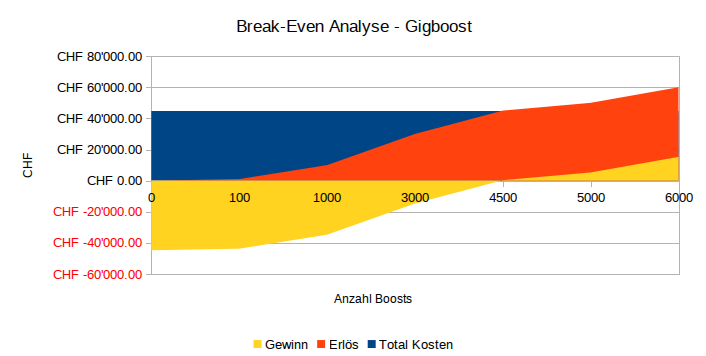
\includegraphics[width=0.95\textwidth]{initialisierung/wirtschaftlichkeit-gigboost.png}
  \caption{Breaz-Even Analyse - Gigboost}
\end{figure}

\clearpage
\subsubsection{Werbung}

Im Modell "Werbung" wird ausgerechnet wieviele aktive Benutzer das Produkt benötigt
um in den nächsten Jahren Gewinn zu erzielen.

Durch Annahme von einem Erlös von \textbf{140.- CHF} pro \textbf{40'0000 Besucher}\footnote{https://www.quora.com/How-much-does-Google-AdSense-pay-for-3-banners-on-a-webpage-per-1-000-views/answer/Manas-Sahu-59} erhalten wir volgendes Bild:

\begin{figure}[!htb]
  \centering
  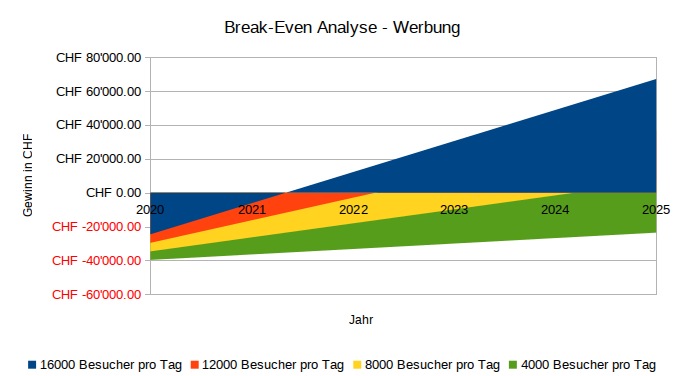
\includegraphics[width=0.95\textwidth]{initialisierung/wirtschaftlichkeit-werbung.png}
  \caption{Break-Even Analyse - Werbung}
\end{figure}

\begin{longtable}[]{@{}lll@{}}
  \toprule
  \textbf{Besucher pro Tag} & \textbf{Erlös pro Tag} & \textbf{Erlös pro Monat}\tabularnewline
  2000                      & 7.- CHF                & 210.- CHF\tabularnewline
  4000                      & 14.- CHF               & 420.- CHF\tabularnewline
  8000                      & 28.- CHF               & 840.- CHF\tabularnewline
  12000                     & 42.- CHF               & 1'260.- CHF\tabularnewline
  16000                     & 46.- CHF               & 1'680.- CHF\tabularnewline
  \bottomrule
  \caption{Werbeeinnahmen pro Besucher}
\end{longtable}

Der Grafik ist zu entnehmen, dass das Produkt bei 8'000 Besucher pro Tag nach ca. 6 Jahren Gewinn erzielt. Bei 12'000 Besucher pro Tag erzielt das Produkt nach bereits 4 Jahren Gewinn und mit 16'000 Beucher pro Tag schon im dritten Jahr.

\chapter{Konzept}

\label{AppendixKonzept}

\section{Zweck des Dokuments}\label{KonzeptZweck}

Das Konzept dient als Anleitung für die Realisierungsphase. Die in der Konzept
erarbeiteten Details müssen in der Realisierung eingehalten un umgesetzt
werden.

\subsection{Teilkonzepte}

Durch die in der Studie gewonnenen Erkentnissen, werden in der Phase Konzept
verschiedene Teilkonzepte erstellt.

Im Teilkonzept «Portalname» wird der Name des Produktes erarbeitet.

Im Teilkonzept «Design- und Bedienkonzept» werden die Ansichten der Applikation
in Mockups umgesetzt. Es werden die Benutzer Use-Cases vom Besucher sowie der
Konzert-Erfasser aufgezeigt.

Im Teilkonzept «Softwarekonzept» werden die Datenflüsse hinter den Mockups
aufgezeigt, sowie die Datenbankstruktur aufgebaut.

Im Teilkonzept «Testkonzept» werden die einzelnen Systemtests aufgelistet sowie
ausgearbeitet wie granular welche Teile der Software getestet werden sollen.

Im letzten Teil des Konzept-Dokuments wird im Fazit dokumentiert, wie und warum
das Konzept von den vorhergehenden Phasen des Projekts abweicht.


\clearpage
\section{Portalname}\label{portalname}

Der Portalname wurde in einer Brainstorming-Session von Damian Senn auf
den Namen \textbf{«Gigpillar»} festgelegt. Der Name ist angelehnt an die Werbepfeiler in
Städten, wo oft Werbeplakate für Konzerte hängen.

Die folgenden Ideen wurden in Betracht gezogen, jedoch war keine Domain mehr
verfügbar oder der Name überzeugte nicht:

\begin{itemize}
  \item{} upto.com («What are you up to?»)
  \item{} up-to.com
  \item{} uptoin.com
  \item{} gigup.com
  \item{} gigsta.com («Gigs to attend»)
  \item{} gigin.com
  \item{} gigsin.com
  \item{} gixin.com («Gigs in»)
  \item{} dualact.com («Loud act»)
  \item{} trecnoc.com («Concert» rückwärts)
\end{itemize}

\clearpage
\section{Design- und Bedienkonzept}\label{design--und-bedienkonzept}

\subsection{Mockups}

\subsubsection{Homepage}

Die Homepage ist die erste Seite, die der Besucher sieht, wenn er/sie die
Applikation direkt über \href{https://gigpillar.com/}{gigpillar.com} aufruft.
Auf den ersten Blick ist die Suche sowie ein grosses Bild (Banner) eines Gigs
zu erblicken. Weiter sind Links zu gängigen Funktionalitäten wie Gig hinzufügen
sowie das Login in einer Navigation erreichbar.

Unter dem Banner werden Gigs in nächster nähe des Besuchers aufgelistet, der
Link «change location» führt weiter zur Suchresultate Seite um den
entsprechenden Filter anzupassen.

\begin{figure}[!htb]
  \centering
  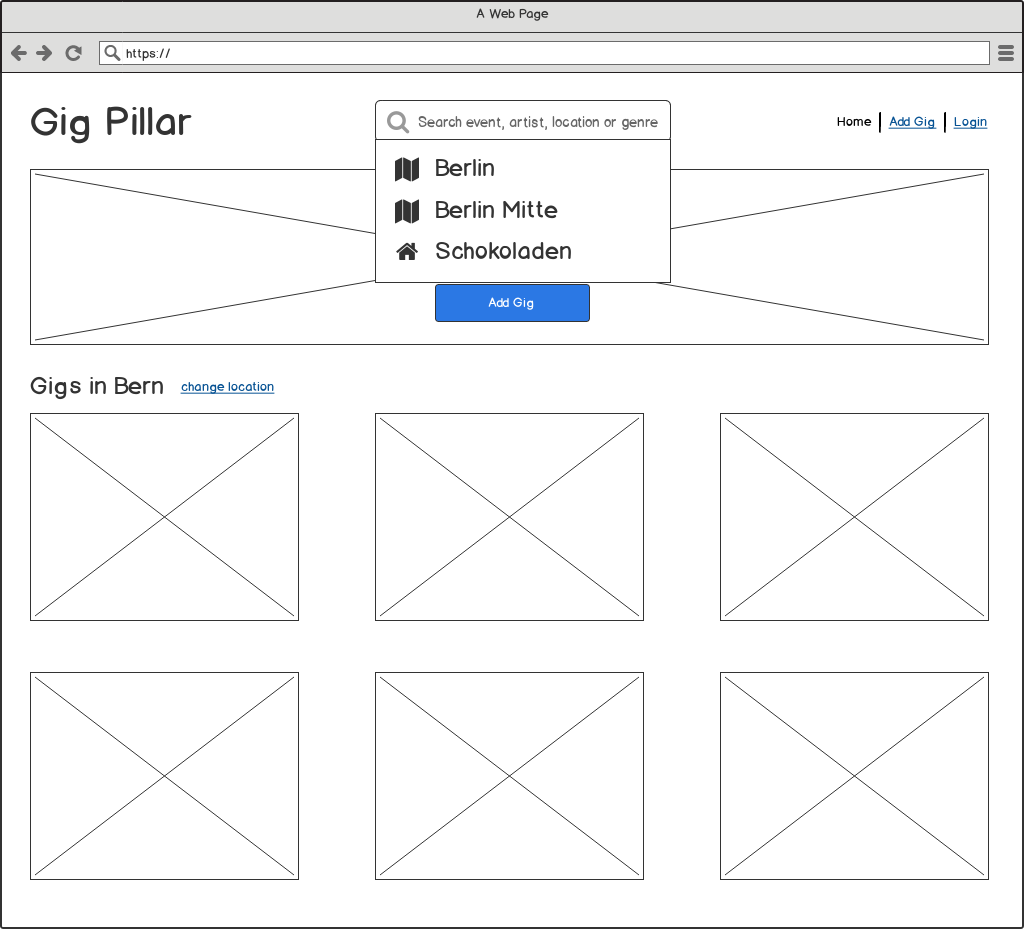
\includegraphics[width=0.95\textwidth]{mockups/homepage.png}
  \caption{Mockup: Homepage}
\end{figure}

\clearpage
\subsubsection{Suchresultate}

Auf der Suchresultate Seite sieht der Benutzer seine Suchresultate der von der
globalen Suchbox ausgelösten Suche. Die Seite bietet weitere Filter an um die
Resultate weiter einzugrenzen.\\

\noindent
Folgende Filter stehen den Benutzern zur Verfügung:

% TODO: This diverges from our search criteria described in the previous phase.

\begin{itemize}
  \tightlist{}
  \item{} Ort
  \item{} Datum von
  \item{} Datum bis
  \item{} Musik Genre
\end{itemize}

\noindent
Das Anwählen eines Suchresultates führt den Benutzer weiter zur detaillierten
Gig Ansicht.

\begin{figure}[!htb]
  \centering
  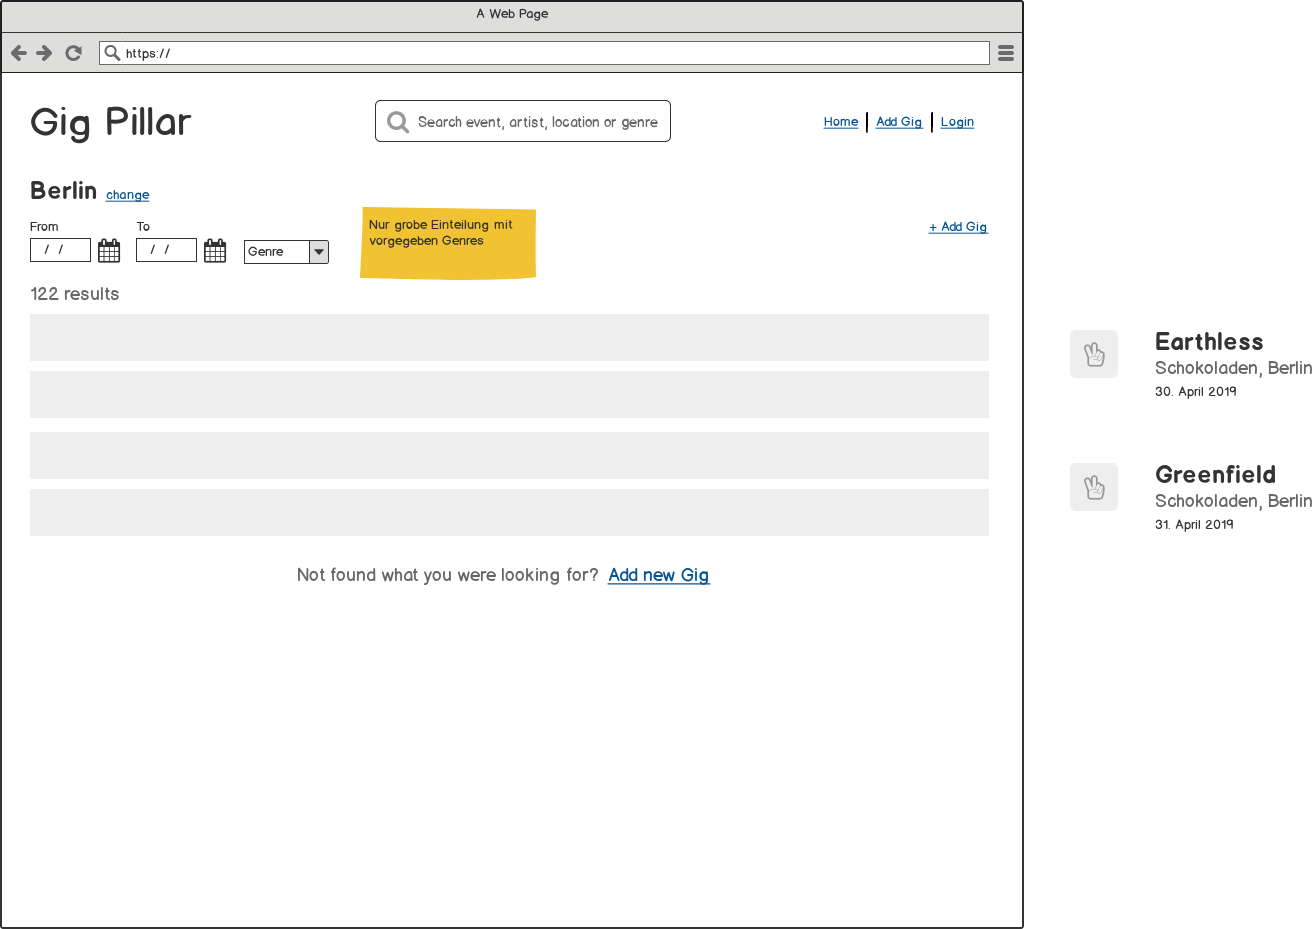
\includegraphics[width=0.95\textwidth]{mockups/search-result.png}
  \caption{Mockup: Suchresultate}
\end{figure}

\clearpage
\subsubsection{Gig Ansicht}

In der Gig Ansicht werden alle Details zu einem Event aufgelistet.

\begin{itemize}
  \tightlist{}
  \item{} Datum des Events
  \item{} Zeit wann das Event beginnt, bzw die Location die Türen öffnet
  \item{} Liste aller Künstler mit optionaler Startzeit
  \item{} Eine Beschreibung des Events
  \item{} Die Adresse der Location mit Link auf Google Maps
\end{itemize}

\noindent
Ausserdem soll es den Benutzern möglich sein, über einen «Add to my calendar»
Link das Event zu seiner Kalender-Applikation zu importieren.

\begin{figure}[!htb]
  \centering
  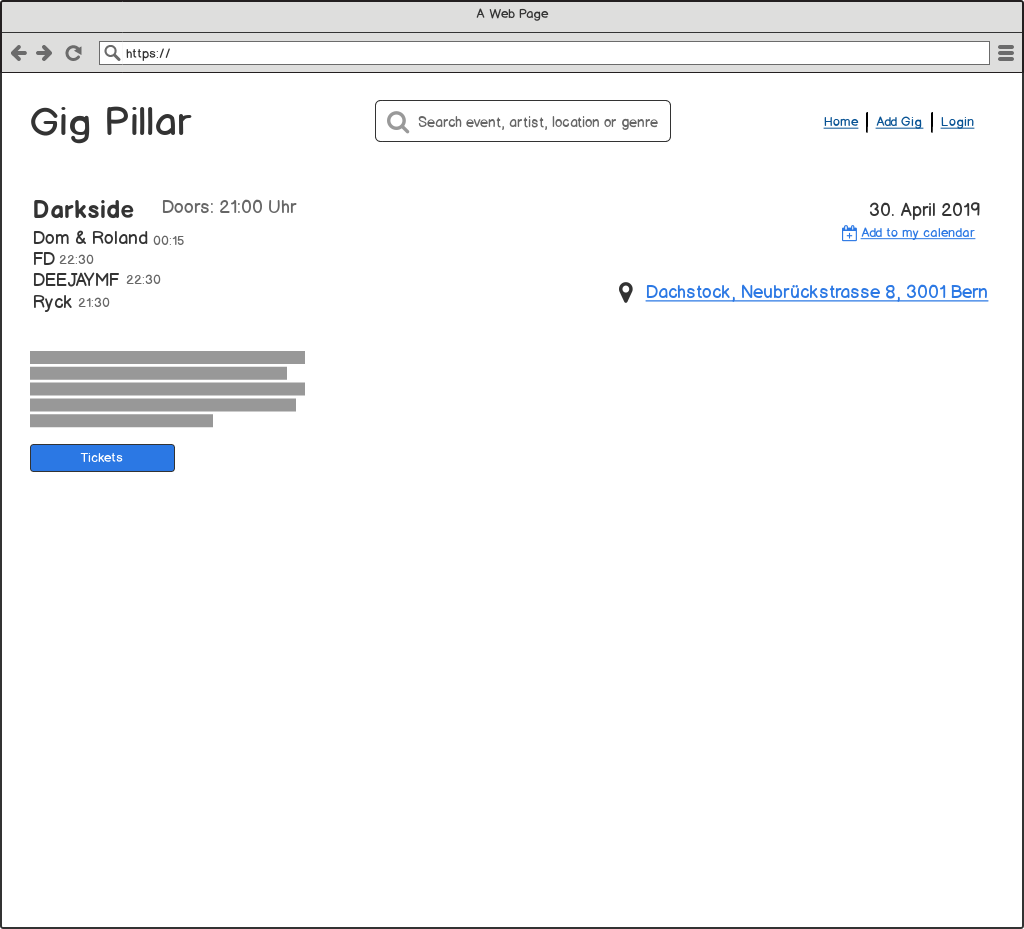
\includegraphics[width=0.95\textwidth]{mockups/event.png}
  \caption{Mockup: Gig Ansicht}
\end{figure}

\clearpage
\subsubsection{Gig erfassen}

Benutzer können Gigs erfassen.\\

\noindent
Folgende Daten sind für einen Gig zu erfassen:

\begin{itemize}
  \tightlist{}
  \item{} Name
  \item{} Bild \textit{(optional)}
  \item{} Location
  \item{} Datum
  \item{} Zeit
  \item{} Eine Liste von Artists mit optionaler Startzeit
  \item{} Beschreibung
  \item{} Link zum Ticketvertreiber
\end{itemize}

\begin{figure}[!htb]
  \centering
  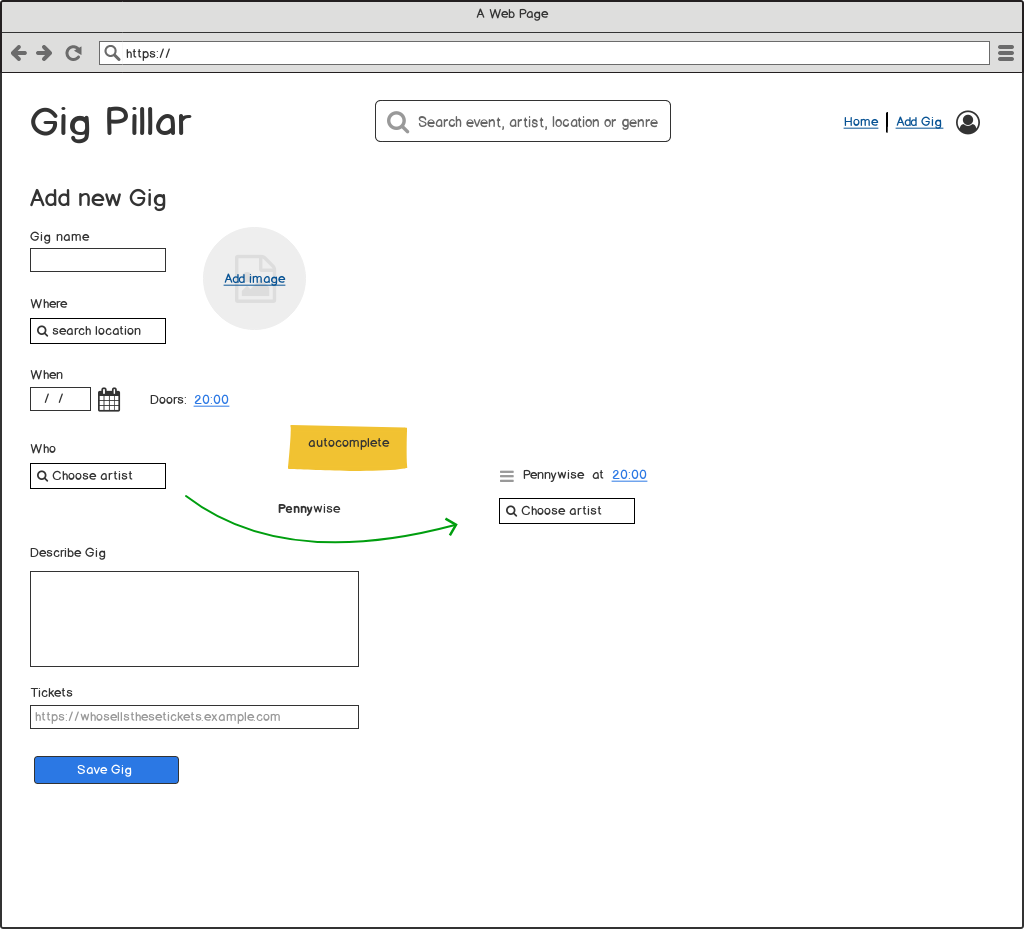
\includegraphics[width=0.95\textwidth]{mockups/add-gig.png}
  \caption{Mockup: Gig erfassen}
\end{figure}

\clearpage
\subsubsection{Benutzerprofil}

Benutzer können ihr eigenes Profil verwalten und folgende Tätigkeiten
verrichten:

\begin{itemize}
  \tightlist{}
  \item{} Anzeigename ändern
  \item{} E-Mail Adresse ändern \textit{(mit E-Mail Bestätigung)}
  \item{} Passwort ändern \textit{(muss vorher altes Passwort bestätigen)}
  \item{} Account löschen \textit{(muss doppelt bestätigt werden!)}
\end{itemize}

\begin{figure}[!htb]
  \centering
  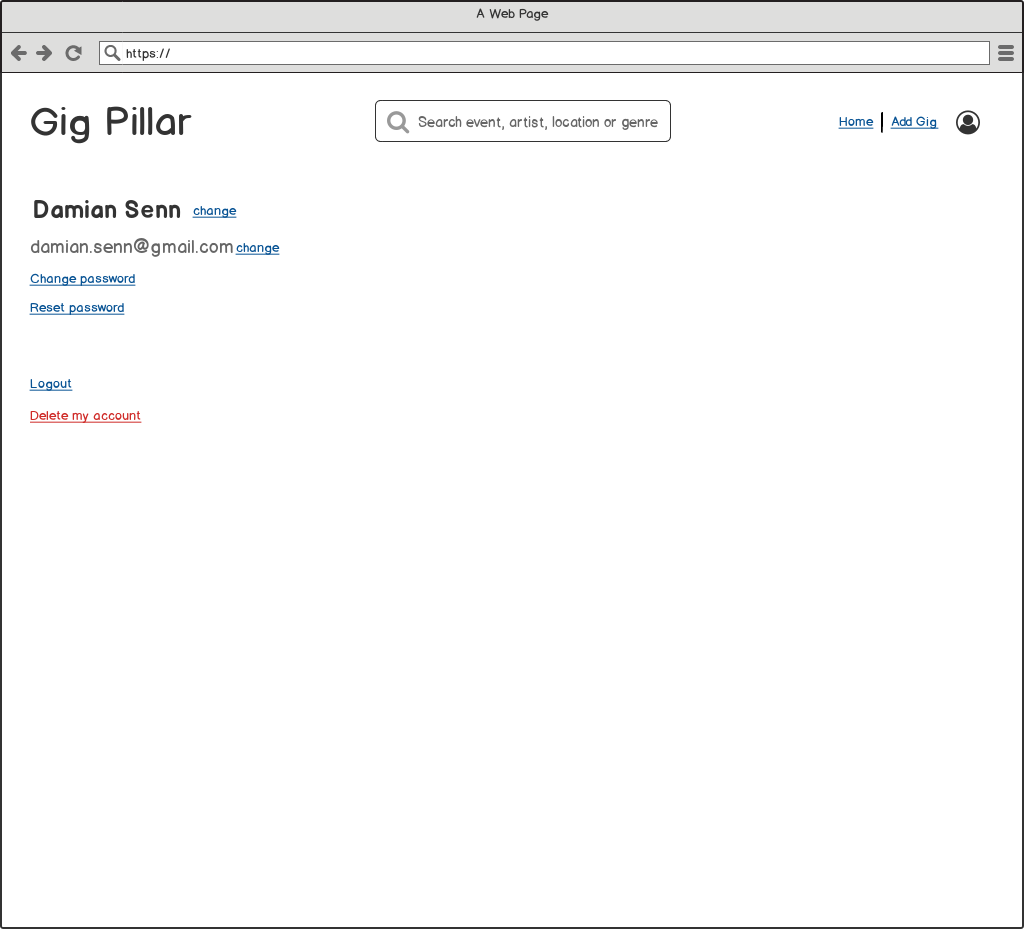
\includegraphics[width=0.95\textwidth]{mockups/profile.png}
  \caption{Mockup: Benutzerprofil}
\end{figure}

\clearpage
\subsection{Genre Filter}\label{genrefilter}

Der Genre Filter soll folgende Werte zur Verfügung stellen.

\begin{itemize}
  \item{} Alternative
  \item{} Blues
  \item{} Classical
  \item{} EDM
  \item{} Hip-Hop
  \item{} Jazz
  \item{} Metal
  \item{} Pop
  \item{} Punk
  \item{} Reggae
  \item{} Rock
\end{itemize}

\clearpage
\section{Softwarekonzept}\label{softwarekonzept}
\subsection{Datenfluss}\label{datenfluss}

\subsubsection{Homepage}\label{datenfluss-homepage}

Die Homepage zeigt den Besuchern Gigs in ihrer Nähe an, dazu muss über eine
GeoIP API die IP-Adresse des Besuchers auf ein Land zurückverfolgt werden.
Dazu wird beim ersten Besuch die GeoIP API abgefragt und das Land des Benutzers
in eine Session geschrieben. Bei weiteren Aufrufen wird das Land direkt aus der
Session bezogen.

%GigPillarWeb
%GigPillarWeb_Session
%GigPillar
%GeoIp
%
%Response = GigPillarWeb./ {
%  if (hasSession) {
%    location = GigPillarWeb_Session.getLocation()
%  } else {
%    location = GigPillarWeb_Session.createSession() {
%      location = GeoIp.getLocation(ip)
%    }
%  }
%
%  Events = GigPillar.getUpcomingEvents(location)
%}

\begin{figure}[!htb]
  \centering
  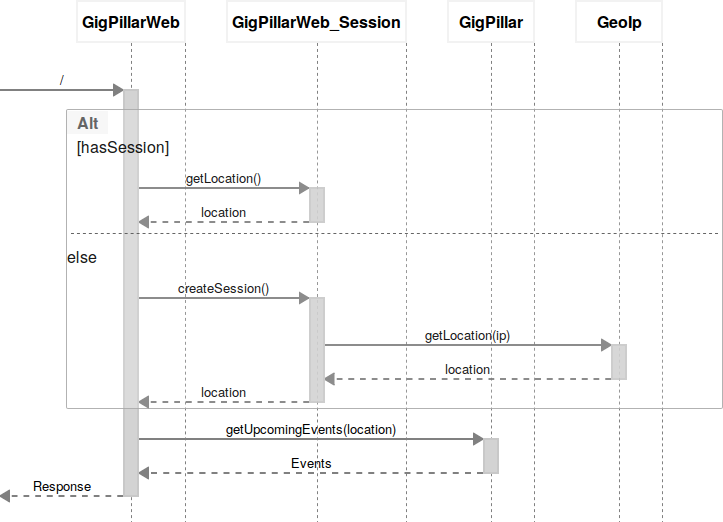
\includegraphics[width=0.95\textwidth]{konzept/datenfluss-homepage.png}
  \caption{Datenfluss: Homepage}
\end{figure}

\clearpage
\subsubsection{Suchfeld}\label{datenfluss-suchfeld}

Das globale Suchfeld hat eine Autocompletion, welche Daten direkt von
der GigPillar Applikation bezieht. Die Daten für Städtenamen wird jedoch von
einer externen Datenquelle, z.B. Google Maps, bezogen.

%GigPillarWeb
%GigPillar
%GoogleMaps
%
%Response = GigPillarWeb./searchCompletion {
%  Cities = GoogleMaps.searchCities(searchParameters)
%  Locations = GigPillar.searchLocations(searchParameters)
%  Genres = GigPillar.searchGenres(searchParameters)
%  Artists = GigPillar.searchArtists(searchParameters)
%  Events = GigPillar.searchEvents(searchParameters)
%}

\begin{figure}[!htb]
  \centering
  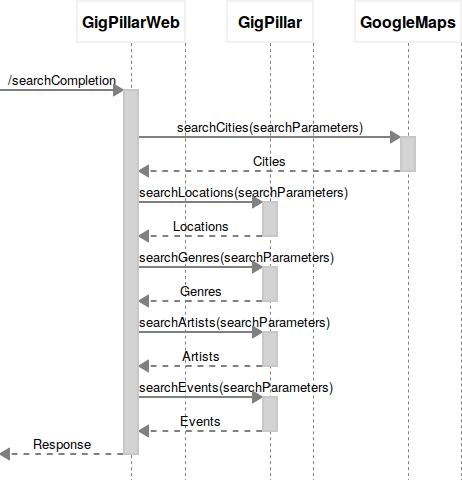
\includegraphics[width=0.95\textwidth]{konzept/datenfluss-suchfeld.png}
  \caption{Datenfluss: Suchfeld}
\end{figure}

\clearpage
\subsubsection{Gig erstellen - Locationfeld}\label{datenfluss-gig-erstellen-locationfeld}

Beim Erstellen eines neuen Gigs, muss eine Location zugewiesen werden. Die
Locations werden über die bereits in GigPillar erfassten Locations sowie über
eine externe Datenquelle, wie z.B. Google Maps, bezogen.

%GigPillarWeb
%GigPillar
%GoogleMaps
%
%Response = GigPillarWeb./locationCompletion {
%  Locations = GigPillar.searchLocations(searchParameters) {
%    Locations = searchLocations(searchParameters)
%    Locations = GoogleMaps.searchLocations(searchParameters)
%  }
%}

\begin{figure}[!htb]
  \centering
  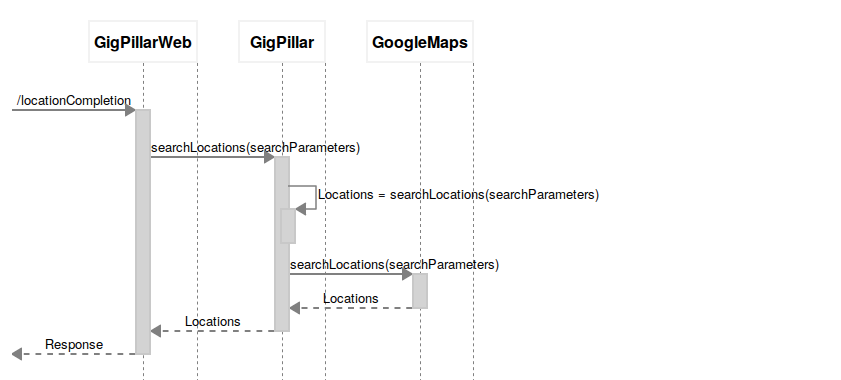
\includegraphics[width=0.95\textwidth]{konzept/datenfluss-locationfeld.png}
  \caption{Datenfluss: Gig erstellen - Locationfeld}
\end{figure}

%TODO:
%\clearpage
%\subsubsection{Gig erstellen}\label{datenfluss-gigerstellen}

\clearpage
\subsubsection{Passwort-Reset}\label{datenfluss-passwort-reset}

Falls ein Benutzer sein Passwort vergessen hat, kann dieser ein neues Passwort
über die Passwort-Reset Funktion setzen. Beim Auslösen eines Passwort-Resets,
wird dem Benutzer ein E-Mail mit einem Link zugeschickt.
Der Passwort-Reset-Link führt den Benutzer auf ein Formular auf welchem er/sie
die Möglichkeit hat, ein neues Passwort zu setzen.

%GigPillarWeb
%GigPillar
%UserEmailClient
%
%Response = GigPillarWeb./passwordReset {
%  GigPillar.sendPasswordResetEmail(email) {
%    GigPillar->UserEmailClient:SMTP
%  }
%}
%
%Redirect = UserEmailClient.clickPasswordResetLink {
%  Response = GigPillarWeb./passwordRestToken
%}
%
%Response = GigPillarWeb./setPassword {
%  GigPillar.setUserPassword(currentUser, password)
%}

\begin{figure}[!htb]
  \centering
  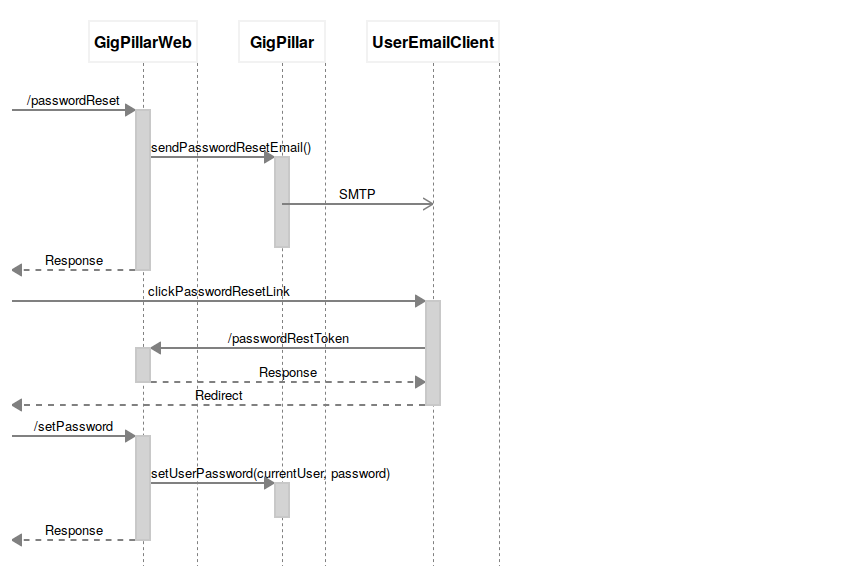
\includegraphics[width=0.95\textwidth]{konzept/datenfluss-passwort-reset.png}
  \caption{Datenfluss: Passwort-Reset}
\end{figure}

\clearpage
\subsection{Datenbankstruktur}\label{datenbankstruktur}

\begin{figure}[!htb]
  \centering
  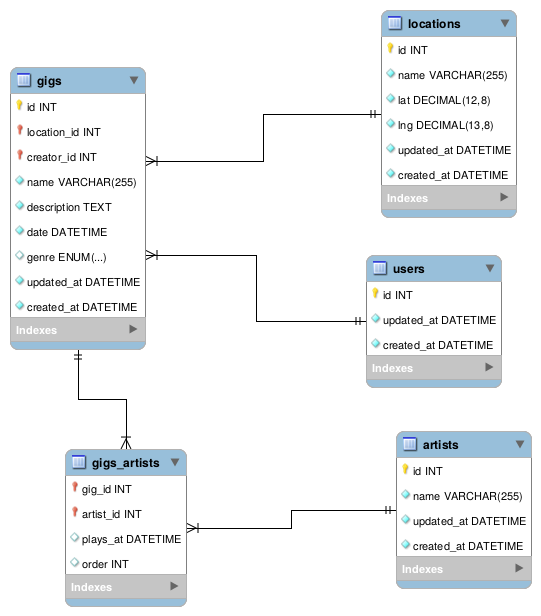
\includegraphics[width=0.95\textwidth]{konzept/erd.png}
  \caption{Entity Relationship Diagram}
\end{figure}

\clearpage
\section{Testkonzept}\label{testkonzept}

\subsection{Unit-Tests}\label{unittests}

% Do ~80% code coverage

\subsection{Visual-Tests}\label{visualtests}

% Do simple screenshot diffing for every screen

\clearpage
\subsection{Akzeptanztests}\label{akzeptanztests}

% TODO: Akzeptanztest basieren auf Anforderungen

\newcounter{acceptancetest}

\NewDocumentCommand{\acceptancetest}{
  O{}
  O{}
  O{\tabularnewline\tabularnewline}
  O{\tabularnewline\tabularnewline\tabularnewline\tabularnewline}
  m
  m
}{
  \begin{longtable}[]{@{}l|p{6cm}p{4cm}@{}}
    \toprule
    \stepcounter{acceptancetest}
    \textbf{Test \arabic{acceptancetest}} & \textbf{Tester:} #1 & \textbf{Datum:} #2 \tabularnewline
    \midrule
    \textbf{Kriterium}                    & \multicolumn{2}{p{10cm}}{#5}\tabularnewline
    \textbf{Erwartetes Ergebnis}          & \multicolumn{2}{p{10cm}}{#6}\tabularnewline
    \midrule
    \textbf{Testergebnis}                 & #3\tabularnewline
    \midrule
    \textbf{Fehlerbeschreibung}           & #4\tabularnewline
    \bottomrule
    \caption{Akzeptanztest \arabic{acceptancetest}}
  \end{longtable}
}

\acceptancetest
  {Es ist möglich nach Konzerten in einem bestimmten Ort zu suchen.}
  {Nach auswählen von «Berlin» in der Suche, werden nur noch Konzerte in Berlin aufgelistet.}

\acceptancetest
  {Es ist möglich eine Suche weiter nach Genre einzuschränken.}
  {Nach auswählen von «Rock» in einem Suchresultat, werden nur noch Rock-Konzerte aufgelistet.}

\clearpage

\acceptancetest
  {Responsive - Homepage}
  {Sieht auf Desktop, Tablet und Mobile gut aus und stellt jeweils alle relevanten Daten dar.}

\acceptancetest
  {Browserkompatibilität - Homepage}
  {Funktioniert in den unterstützten Browsern.}

\clearpage

\acceptancetest
  {Responsive - Suche}
  {Sieht auf Desktop, Tablet und Mobile gut aus und stellt jeweils alle relevanten Daten dar.}

\acceptancetest
  {Browserkompatibilität - Suche}
  {Funktioniert in den unterstützten Browsern.}

\clearpage

\acceptancetest
  {Responsive - Gig Ansicht}
  {Sieht auf Desktop, Tablet und Mobile gut aus und stellt jeweils alle relevanten Daten dar.}

\acceptancetest
  {Browserkompatibilität - Gig Ansicht}
  {Funktioniert in den unterstützten Browsern.}

\clearpage

\acceptancetest
  {Responsive - Login}
  {Sieht auf Desktop, Tablet und Mobile gut aus und stellt jeweils alle relevanten Daten dar.}

\acceptancetest
  {Browserkompatibilität - Login}
  {Funktioniert in den unterstützten Browsern.}

\clearpage

\acceptancetest
  {Responsive - Registrierung}
  {Sieht auf Desktop, Tablet und Mobile gut aus und stellt jeweils alle relevanten Daten dar.}

\acceptancetest
  {Browserkompatibilität - Registrierung}
  {Funktioniert in den unterstützten Browsern.}

\clearpage

\acceptancetest
  {Responsive - Gig erfassen}
  {Sieht auf Desktop, Tablet und Mobile gut aus und stellt jeweils alle relevanten Daten dar.}

\acceptancetest
  {Browserkompatibilität - Gig erfassen}
  {Funktioniert in den unterstützten Browsern.}

\clearpage

\acceptancetest
  {Gig erfassen}
  {Folgende Daten können erfasst werden:
  \begin{itemize}
    \tightlist{}
    \item{} Name
    \item{} Bild
    \item{} Location
    \item{} Datum
    \item{} Zeit
    \item{} Künstler mit optinaler Start-Zeit
    \item{} Beschreibung
    \item{} Link zum Ticketvertreiber
  \end{itemize}}

\acceptancetest
  {Neue Gigs tauchen in der Suche auf.}
  {Der neu erstellte Gig taucht in der Suche auf.}

\clearpage

\acceptancetest
  {Responsive - Benutzerprofil}
  {Sieht auf Desktop, Tablet und Mobile gut aus und stellt jeweils alle relevanten Daten dar.}

\acceptancetest
  {Browserkompatibilität - Benutzerprofil}
  {Funktioniert in den unterstützten Browsern.}

\clearpage

\acceptancetest
  {Responsive - Passwort-Reset}
  {Sieht auf Desktop, Tablet und Mobile gut aus und stellt jeweils alle relevanten Daten dar.}

\acceptancetest
  {Browserkompatibilität - Passwort-Reset}
  {Funktioniert in den unterstützten Browsern.}

\clearpage

\acceptancetest
  {Security - Suche}
  {Das Suchfeld ist resistent gegen XSS und SQL-Injection}

\acceptancetest
  {Security - Login}
  {Das Login ist resistent gegen XSS und SQL-Injection}

\clearpage

\acceptancetest
  {Security - Benutzerprofil}
  {Das Benutzerprofil ist resistent gegen XSS und SQL-Injection}

\acceptancetest
  {Security - Gig erfassen}
  {Das Gig erfassen Formular ist resistent gegen XSS und SQL-Injection}

\clearpage
\section{Fazit}\label{konzept-fazit}

\subsection{Probleme}

% Abweichung "Filter-System" in Suche?

\subsection{Machbarkeit}

% Google Maps API?

\subsection{Wirtschaftlichkeit}

% Änderung an Aufwand?

\subsection{Erweiterbarkeit}

% FB Events etc?

\subsection{Projektplan}

\chapter{Arbeitsjournal}

\label{AppendixArbeitsjournal}

\section{Sonntag 3. März}\label{sonntag-3.-muxe4rz}

2h:

\begin{itemize}
  \tightlist
  \item
        Vorbereitung Kick-off
  \item
        Abgrenzung erweitern
  \item
        Grobe Anforderungen
  \item
        Auflistung möglicher Variantenentscheide
  \item
        TODO ergänzt
\end{itemize}

\section{Dienstag 5. März}\label{dienstag-5.muxe4rz}

2h:

\begin{itemize}
  \tightlist
  \item
        Vorbereitung Kick-off
\end{itemize}

\section{Mittwoch 6. März}\label{mittwoch-6.muxe4rz}

3h:

\begin{itemize}
  \tightlist
  \item
        Vorbereitung Sitzungszimmer
  \item
        Kick-off Meeting
\end{itemize}

4h:

\begin{itemize}
  \tightlist
  \item
        An Projektauftrag arbeiten - Auftraggeber geändert nach Empfehlung
        von Marc Aeby
\end{itemize}

\section{Samstag 9. März}\label{samstag-9.muxe4rz}

2h:

\begin{itemize}
  \tightlist
  \item
        An Studie/Pflichtenheft arbeiten
\end{itemize}

\section{Dienstag 12. März}\label{dienstag-12.muxe4rz}

2h:

\begin{itemize}
  \tightlist
  \item
        PDF Generierung und Ordnerstruktur angepasst
\end{itemize}

\section{Samstag 16. März}\label{samstag-16.muxe4rz}

3h:

\begin{itemize}
  \tightlist
  \item
        Projektplan von gantt nach ods migrieren
\end{itemize}

\section{Dienstag 19. März}\label{dienstag-19.muxe4rz}

0.5h:

\begin{itemize}
  \tightlist
  \item
        Projektplan in Berichtanhang angehängt
\end{itemize}

\section{Mittwoch 27. März}\label{mittwoch-27.muxe4rz}

1.5h:

\begin{itemize}
  \tightlist
  \item
        Projektplan an korrekte HERMES 5 Struktur angepasst
  \item
        Titelblatt von Ilias hinzugefügt
  \item
        Termin am 12.04.2019 mit Joshua Schär für einen Screendesign-Workshop abgemacht
\end{itemize}

\section{Sonntag 31. März}\label{sonntag-31.muxe4rz}

5h:

\begin{itemize}
  \tightlist
  \item
        Projektziele erweitert
  \item
        Anforderungskatalog erweitert
\end{itemize}

\section{Sonntag 31. März}\label{sonntag-31.muxe4rz}

8h:

\begin{itemize}
  \tightlist
  \item
        Definitive Projektziele definiert
  \item
        Anforderungskatalog fertig gestellt
  \item
        Gesamte Berichtstruktur ausgelegt, Ziele und Abgrenzungen in Bericht
        hinterlegt und referenziert
\end{itemize}

\section{Freitag 5. April}\label{freitag-5.april}

2h:

\begin{itemize}
  \tightlist
  \item
        An Studie weiter gearbeitet
  \item
        Variantenkriterien definiert
\end{itemize}

\section{Samstag 6. April}\label{samstag-6.april}

4h:

\begin{itemize}
  \tightlist
  \item
        An Studie weiter gearbeitet
  \item
        Variantenbeschreibungen erstellt
  \item
        Variantenbewertungen
\end{itemize}

\section{Mittwoch 10. April}\label{mittwoch-10.april}

2h:

\begin{itemize}
  \tightlist
  \item
        Brainstorming für Portalnamen
\end{itemize}

\section{Freitag 12. April}\label{freitag-12.april}

12h:

\begin{itemize}
  \tightlist
  \item
        Screens definiert
  \item
        Mit Joshua Schär an Mockups gearbeitet
\end{itemize}

\section{Samstag 13. April}\label{samstag-13.april}

12h:

\begin{itemize}
  \tightlist
  \item
        Risiko Management
  \item
        Variantenbeschreibungen angepasst/erweitert
  \item
        Projektauftrag
\end{itemize}

\section{Sonntag 14. April}\label{sonntag-14.april}

8h:

\begin{itemize}
  \tightlist
  \item
        Wirtschaftlichkeit
  \item
        Projektauftrag
\end{itemize}

\section{Montag 15. April}\label{montag-15.april}

2h:

\begin{itemize}
  \tightlist
  \item
        Initiales Datenbankschema basierend auf Mockups
\end{itemize}

\section{Mittwoch 17. April}\label{mittwoch-17.april}

0.5h:

\begin{itemize}
  \tightlist
  \item
        Zwischen-Meeting in Planung in richtiger KW eingetragen.
  \item
        Biweekly Reports in Anhang eingefügt.
\end{itemize}

\section{Freitag 19. April}\label{freitag-19.april}

10h:

\begin{itemize}
  \tightlist
  \item
        Alle Mockups detailreicher beschrieben.
  \item
        Kleinere Mockup Anpassungen.
  \item
        Software Konzept mit Datenfluss-Charts beschrieben
\end{itemize}

\section{Sonntag 21. April}\label{sonntag-21.april}

10h:

\begin{itemize}
  \tightlist
  \item
        Mockup Beschreibungen
  \item
        Datenbankschema
  \item
        Mit Testkonzept begonnen
\end{itemize}

\section{Montag 22. April}\label{montag-22.april}

2h:

\begin{itemize}
  \tightlist
  \item
        An Testkonzept gearbeitet
  \item
        An Datenbankschema gearbeitet
\end{itemize}

\section{Dienstag 23. April}\label{dienstag-23.april}

6h:

\begin{itemize}
  \tightlist
  \item
        Zwischenmeeting Präsentation erstellt
  \item
        An Datenbankschema gearbeitet
\end{itemize}

\section{Mittwoch 24. April}\label{mittwoch-24.april}

3h:

\begin{itemize}
  \tightlist
  \item
        Zwischenmeeting
  \item
        Initiales Projektsetup erstellt
\end{itemize}

\section{Mittwoch 1. Mai}\label{mittwoch-1.mai}

14h:

\begin{itemize}
  \tightlist
  \item
        Begin an HTML-Prototypen
\end{itemize}

\section{Sonntag 5. Mai}\label{sonntag-5.mai}

11h:

\begin{itemize}
  \tightlist
  \item
        An HTML-Prototypen gearbeitet
  \item
        Initiale Login Implementation
\end{itemize}

\section{Montag 6. Mai}\label{montag-6.mai}

12h:

\begin{itemize}
  \tightlist
  \item
        Script zum erstellen von Benutzern
  \item
        Registrierungsprozess implementiert
  \item
        Session Management eingerichtet
  \item
        Berechtigungssystem definiert
  \item
        Mit Erfassungsformular für Gigs begonnen
\end{itemize}

\section{Dienstag 7. Mai}\label{dienstag-7.mai}

1h:

\begin{itemize}
  \tightlist
  \item
        Unit-Tests für Gigs
\end{itemize}

\section{Mittwoch 8. Mai}\label{mittwoch-8.mai}

10h:

\begin{itemize}
  \tightlist
  \item
        An Gig Erfassungsformular gearbeitet, diverse Problematiken mit
        Phoenix Formular sowie Datenbankbeziehungen aufgetreten.
  \item
        Google Places API angebunden für Location Autocomplete
  \item
        Generische Suchbox in HTML/JavaScript implementiert
\end{itemize}

\section{Donnerstag 9. Mai}\label{donnerstag-9.mai}

11h:

\begin{itemize}
  \tightlist
  \item
        JavaScript, HTML und CSS Optimierungsplugins installiert
  \item
        Location Autocomplete fertiggestellt
  \item
        Künstlerfeld für Gigs implementiert
  \item
        Fehlermeldungen für invalide Felder eingefügt
  \item
        Bildinputfeld implementiert
  \item
        Debugging von diversen Probleme im Zusammenhang mit Datenbankrelationen
        für das Gig erfassen/updaten Formular
\end{itemize}

\section{Freitag 10. Mai}\label{freitag-10.mai}

1h:

\begin{itemize}
  \tightlist
  \item
        Dropdown Element implementiert
\end{itemize}

\section{Samstag 11. Mai}\label{samstag-11.mai}

13h:

\begin{itemize}
  \tightlist
  \item
        Dropdown Element implementiert
  \item
        Debugging von diversen Probleme im Zusammenhang mit Datenbankrelationen
        für das Gig erfassen/updaten Formular
\end{itemize}

\section{Sonntag 12. Mai}\label{sonntag-12.mai}

7h:

\begin{itemize}
  \tightlist
  \item
        Bildupload für Gigs
  \item
        Begin der Implementation der Suche
\end{itemize}

\section{Montag 13. Mai}\label{montag-13.mai}

10h:

\begin{itemize}
  \tightlist
  \item
        Bilder resizing für Gigs
  \item
        Besucher Location mit GeoIP auflösen
  \item
        Diverse kleinere Bugfixes
  \item
        Gig-Detail Ansicht implementiert
\end{itemize}

\section{Dienstag 14. Mai}\label{dienstag-14.mai}

14h:

\begin{itemize}
  \tightlist
  \item
        Browser-Tests für Gig erstellen, Registrierung, Login und Suche
  \item
        Location Autocomplete Sessiontoken hinzugefügt
  \item
        Realisierungsdokumentation
\end{itemize}

\section{Mittwoch 15. Mai}\label{mittwoch-15.mai}

15h:

\begin{itemize}
  \tightlist
  \item
        Realisierungsdokumentation
  \item
        Bericht schreiben
\end{itemize}


%----------------------------------------------------------------------------------------
%	BIBLIOGRAPHY
%----------------------------------------------------------------------------------------

\printbibliography[heading=bibintoc]

%----------------------------------------------------------------------------------------

\end{document}
